\documentclass[50pt]{report}
\usepackage[Lenny]{fncychap}
\usepackage[T1]{fontenc}
\usepackage[french]{babel}
\usepackage{amsmath}
\usepackage{amsfonts}
\usepackage{amssymb}
\usepackage{fancyhdr}
\usepackage{amsthm}
\usepackage{lettrine}
\usepackage{xcolor}
\usepackage{float}
 \numberwithin{equation}{section} %% Comment out for sequentially-numbered
 \numberwithin{figure}{section} %% Comment out for sequentially-numbered
 \newtheorem{theo}{Th\'eor\`eme}[section]
 \newtheorem{defi}[theo]{D\'efinition}
 \newtheorem{prop}[theo]{Proposition} %%Delete [theo] to re-start numbering
 \newtheorem{exem}[theo]{Exemple}
 \newtheorem{exer}[section]{Exercise}%%Delete [section] for sequential numbering
 \newtheorem{rema}[theo]{Remarque}
 \newtheorem{lemm}[theo]{Lemme} %%Delete [theo] to re-start numbering
 \newtheorem{coro}[theo]{Corollaire} %%Delete [theo] to re-start numbering
\usepackage{fullpage}
\usepackage{graphicx}
\pagestyle{fancy}
\renewcommand{\headrulewidth}{0.4pt}
\fancyhead[EL]{\thepage}
\fancyhead[OR]{\thepage}
\headsep = 20pt
\begin{document}

\begin{titlepage}

    \begin{center}

\noindent {\large \textbf{UNIVERSITÉ MOHAMMED V de Rabat}} \\
\vspace*{0.3cm}
\noindent {\Huge \textbf{Faculté des Sciences }} \\
\vspace*{1cm}

\includegraphics[scale=.30]{LogoFsr.png}
\vspace*{1cm}




\noindent \LARGE \textbf{Département d'Informatique}
\vspace*{.5cm}



\noindent \Large \textbf{Filière Licence fondamentale \\ en Sciences Mathématiques et Informatique}
\vspace*{1cm}


\noindent \Huge \fcolorbox{black}{lightgray}{\textbf{\begin{minipage}{\textwidth} % %\hfill
\begin{center}
PROJET DE FIN D'ÉTUDES
\end{center}
%\hfill
\end{minipage}}} \\
\vspace*{1cm}


\vspace*{0.4cm}
\noindent \large {intitulé :}

\vspace*{0.8cm}
\noindent {\Large \textbf{Application Médicale mobile}} \\
\vspace*{0.3cm}
\noindent \Large Présenté par: \\  \textsc{CHEMMAKHA MOHAMMED \item FILALI TAHA} \\
\vspace*{0.2cm}


\vspace*{0.2cm}
\noindent \large soutenu le 01 Juillet 2019 devant le Jury\\
\vspace*{0.5cm}
\end{center}


\noindent \large
\begin{tabular}{lll}

Mme ZITI  Soumia  &  Professeur à la Faculté des Sciences - Rabat   & \textit{Présidente} \\
M BENKAOUA  Yahya   &  Professeur à la Faculté des Sciences - Rabat & \textit{Encadrant}	\\
Mme OMARY  Fouzia   &  Professeur à la Faculté des Sciences - Rabat & \textit{Examinatrice}  \\
Mme TRICHNI  Soumia    &  Professeur à la Faculté des Sciences - Rabat & \textit{Examinatrice}


\end{tabular}

\vfill
\begin{center}
Année universitaire 2018-2019
\end{center}
\end{titlepage}
\sloppy

\titlepage

\newpage

\chapter*{Remerciement}

\addcontentsline{toc}{chapter}{Remerciements}
\begin{large}
Au terme de ce projet nous tenons à remercier infiniment tous les enseignants et
administrateurs de la faculté des sciences. \\


Nos vifs remerciements au Professeur YAHYA BENKAOUZ , qui a gardé un oeil attentif sur le déroulement du projet en donnant des remarques constructives. Nous le remercions pour sa disponibilité et son aide précieuse et cela a été un plaisir de travailler sous sa directive. \\

Nous exprimons aussi nos remerciements aux membres du jury pour l’intérêt qu’ils ont porté à notre recherche en acceptant d’examiner notre travail .\\
Enfin, nous tenons également à remercier toutes les personnes qui ont participé de près ou de loin à la réalisation de ce travail.
\end{large}

\newpage
\chapter*{Dédicaces}

\begin{description}
  \item[A nos chers parents] : \\ \\ Que nulle dédicace ne puisse exprimer ce que nous leurs doit, pour leur bienveillance, leur
affection et leur soutien... Trésors de bonté, de générosité et de tendresse, en témoignage de
nos profonds amours et nos grandes reconnaissances « Que Dieu vous garde ». 
\vspace{1cm}
  \item[A nos chères sœurs et nos frères] : \\  \\ En témoignage de nos sincères reconnaissances pour les efforts qu’ils ont consenti pour
l’accomplissement de ce projet. On leur dédie ce modeste travail en témoignage de notre
grand amour et notre gratitude infinie.
A tous nos amis, Pour leur aide et leur soutien moral durant l’élaboration du travail de fin d’études. 
\vspace{1cm}
  \item[A toute nos Familles]  . \\ \\
  \vspace{1cm}
   \item[ A tous ceux dont l’oubli du nom n’est guère celui du cœur...]  . \\ \\
\end{description}





 




\newpage
\chapter*{Résume}
{\large
De nos jours, les technologies de l’information ont envahi tous les domaines y compris education, transport, logistique, sport, etc. \\
L’objectif de ce projet est de tirer profit des facilités offertes par les technologies de l’information pour l’amélioration des services médicaux. \\
Plus précisément, le but est d’améliorer l’interaction entre les médecins et les patients. Cet amélioration est assuré via la mise en place
d’une application mobile permettant aux médecins de bien gérer et suivre l’état de santé de leurs patients. Au niveau des patients, l’application
leur permettra d’avoir toujours un accès à leurs dossiers médicales. \\

Dans ce présent rapport, nous allons décrire les fonctionnalités de l’application en question, ainsi que le processus de développement suivie. Au niveau technologique, le projet a été implémenté en Java sous forme d’une application Android avec une base de données nonSQL Firebase.
}
\addcontentsline{toc}{chapter}{Résume}

\vspace{3cm}

{\large\textbf{Mots-clés:}}
e-health, Dossier médicale, Application mobile, JAVA, ANDROID, Firebase


\newpage

\chapter*{Abstract}
{\large

Nowadays, information technologies have invaded all areas including education, transport, logistics, sports, etc. \\
The objective of this project is to take advantage of the facilities offered by information technologies to enhance e-health services. \\
More specifically, the goal is to improve the interaction between physicians and patients. This improvement is ensured by setting up
a mobile application that allows physicians to properly manage and monitor the health status of their patients. At the patient level, the application
will allow them to always have access to their medical records. \\

In this report, we will describe the features of the application, as well as the considered development process. At the technological level, the project was implemented in Java as an Android application with a nonSQL Firebase database.
}

\addcontentsline{toc}{chapter}{Abstract}
\vspace{3cm}
{\large\textbf{Keywords:}}
Keywords: e-health, Medical record, Mobile App, JAVA, ANDROID, Firebase



\begin{large}
\tableofcontents
\end{large}

\newpage

\listoffigures


\include{Introduction}

\newpage

\chapter{Introduction générale}
{\large


Le marché des technologies a connu une énorme évolution ces dernières années et avec
l'intégration de l'internet il y a eu des changements sur la façon et la rapidité d’accès aux
informations. Plusieurs secteurs se sont adaptés à ce changement et encore plus ont vu le
jour pour satisfaire ces nouveaux clients. \\\\
% Le domaine  de couverture social représente l'un des domaines qui connaissent un nombre énorme de citoyen
% et qui souffrent pour les satisfaire. Ils doivent alors proposer leurs services d’une façon
% plus rapide et sécurisé mais aussi à distance,
% afin de pouvoir éviter la congestion dans les
% établissements d'enregistrement social pour le Maroc.
% \\ \\
Avec l’apparition des appareils mobiles, comme les smartphones et les tablettes qui ont
connu une révolution technologique, il est devenu facile pour un établissement de registre social pour le Maroc(CNSS ...) de gérer ce
conflit par proposer une application mobile capable de procurer des services
indispensables rapidement et à tout moment (Interaction avec les citoyens bénéficiaires, notification des citoyens de toute modification dans la situation ...)
.\\ \\Notre projet consiste à développer une application Mobile/Web de register social pour le Maroc  qui
propose de nombreuses fonctionnalités pour le citoyen ainsi que pour l'employé qui peut
consulter et modifier les registres sociaux
 des citoyens facilement.\\ \\
 Le Registre social est un système robuste d’identification et d’enregistrement de la population  ainsi qu’un outil de coordination des programmes d’assistance sociale dans le pays. Il permet d’assurer l’unicité de l’identité et le suivi de l’évolution des conditions socioéconomiques des ménages vulnérables.\\\\
Le rapport de ce projet se divise en  quatre chapitres principaux, le premier est pour détailler l'étude conceptuelle du projet par des  diagrammes d'UML avec  la descriptive de chaque diagramme
, le deuxième un aperçu sur l'ensemble des outils, framework et langages utilisés
  et le troisième chapitre sert des imprimes d'écran de l'application réalisée. Finalement le quatrième chapitre est un rappel de ce qui a été réalisé au niveau de ce projet et les fonctionnalités qui peuvent être ajouté ou amélioré.\\

}
\newpage 
\chapter{Étude générale de projet}
\section{Contexte de projet}
         Dans le Maroc et surtout pour la gestion de registre social on trouve plusieurs employés qui gèrent les travaux des citoyens mais ça nécessite du temps, et la majorité confrontent des difficultés au niveau du déplacement, la perte du temps … .\\\\
         En ces temps de crise, le « ciblage » constitue une pratique primordiale qui vise à promouvoir une croissance et redistribuer la richesse afin de poursuivre des objectifs d’équité sociale. Pour atteindre ces derniers, il faut créer un registre unique permettant d’identifier et de concentrer les services sur les populations les plus nécessiteuses.\\\\ 
       Le domaine de couverture social représente l’un des domaines qui connaissent un nombre énorme de citoyen et qui souffrent pour les satisfaire. Ils doivent alors proposer leurs services d’une façon plus rapide et sécurisé mais aussi à distance, afin de pouvoir éviter la congestion dans les établissements d’enregistrement social pour le Maroc.

% \subsection*{}
% \chapter*{L'objectif de l'application}
% \chapter*{Spécification détaillée}
\section{Spécification détaillée}
\subsection*{}
% {\large
Au cours des dernières années, avec la transformation numérique, l’industrie de la couverture social  a connu des changements majeurs. Un changement évident est la transition des documents papier aux enregistrements numériques par les établissements des regitres sociaux et d’autres installations. \\

Notre application registre social pour le Maroc permet aux employés  d'enregistrer les opérations  des citoyens et aussi les citoyens peuvent consulter leur dossier social et  d’effectuer toutes les opérations
financières. \\\\\\
\subsection*{}
Les fonctionnements de notre application sont :\vspace*{0.5cm}
\begin{itemize}
  \item[$\bullet$] Les principales utilisateurs de l'application sont les citoyens et les employés.\\
  
   \item[$\bullet$] Un employé peut ouvrir un compte d'affiliation à la CNSS.\\
  \item[$\bullet$] Un citoyen peut consulter son dossier social (situation  avec l’organisem de retraite , couverture médicale, …).\\
%   \item[$\bullet$] Un médecin peut apporter des modifications aux dossiers médicaux de ces patients.
  \item[$\bullet$] L'application doit permettre sécuriser et distribuer des données\\

%   \item[$\bullet$] L'application doit permettre le suivie des changements des paramètres vitaux d'un patient donné par son médecin traitant. (Pour l'instant, vous considérez qu'on dispose au préalable des paramètres vitaux des patients).

   \item[$\bullet$]  Les employées doivent être notifier si l'une des opérations financières à effectuer par le citoyen.\\
  \item[$\bullet$]  Les citoyens et les employées doivent s'authentifier pour accéder à l'application.\\
   \item[$\bullet$] L'application Il permet de  contribuer à la simplification des démarches administratives liées aux services fournis aux citoyen
   \\
   \item[$\bullet$] L’application 
 suivie tous les  changements  financières à effectuer par le citoyen.
%   \item[$\bullet$]  Un médecin peut inviter un patient à partager son dossier médical. Puis, le patient accepte ou non le partage de son dossier.
%   \item[$\bullet$]  Pour un diagnostic donné, un médecin peut inviter d'autres médecins collaborateurs pour s'entre-aider à étudier le cas d'un patient donné.
%   \item[$\bullet$]  Pour un diagnostic donné, un médecin peut inviter d'autres médecins collaborateurs pour s'entre-aider à étudier le cas d'un patient donné.
%   \item[$\bullet$] Lorsque un médecin consulte le dossier médical d'un patient, il faut qu'il aie la possibilité de voir seulement les paramètres vitaux d'une (ou plusieurs) maladie(s) donnée(s).

\end{itemize}
\newpage
\subsection*{}
% \chapter*{L'objectif de l'application}
% \chapter*{Spécification détaillée}
% \section{Système existant}
\section{les regitres sociaux existants}
\subsection*{}
\textbf{La sécurité sociale en Suède} [1] : Est  l’une des composantes du système de protection sociale suédois et se compose de diverses assurances sociales gérées par l’Agence nationale d’assurance sociale (suédoise; Försäkringskassan), ainsi que de prestations sociales fournies sur une base de besoins par les municipalités locales. Ils sont les principaux canaux de redistribution d’environ 48\% du PIB suédois sous forme de revenu imposé.  

\begin{figure}[!h]
  \centering
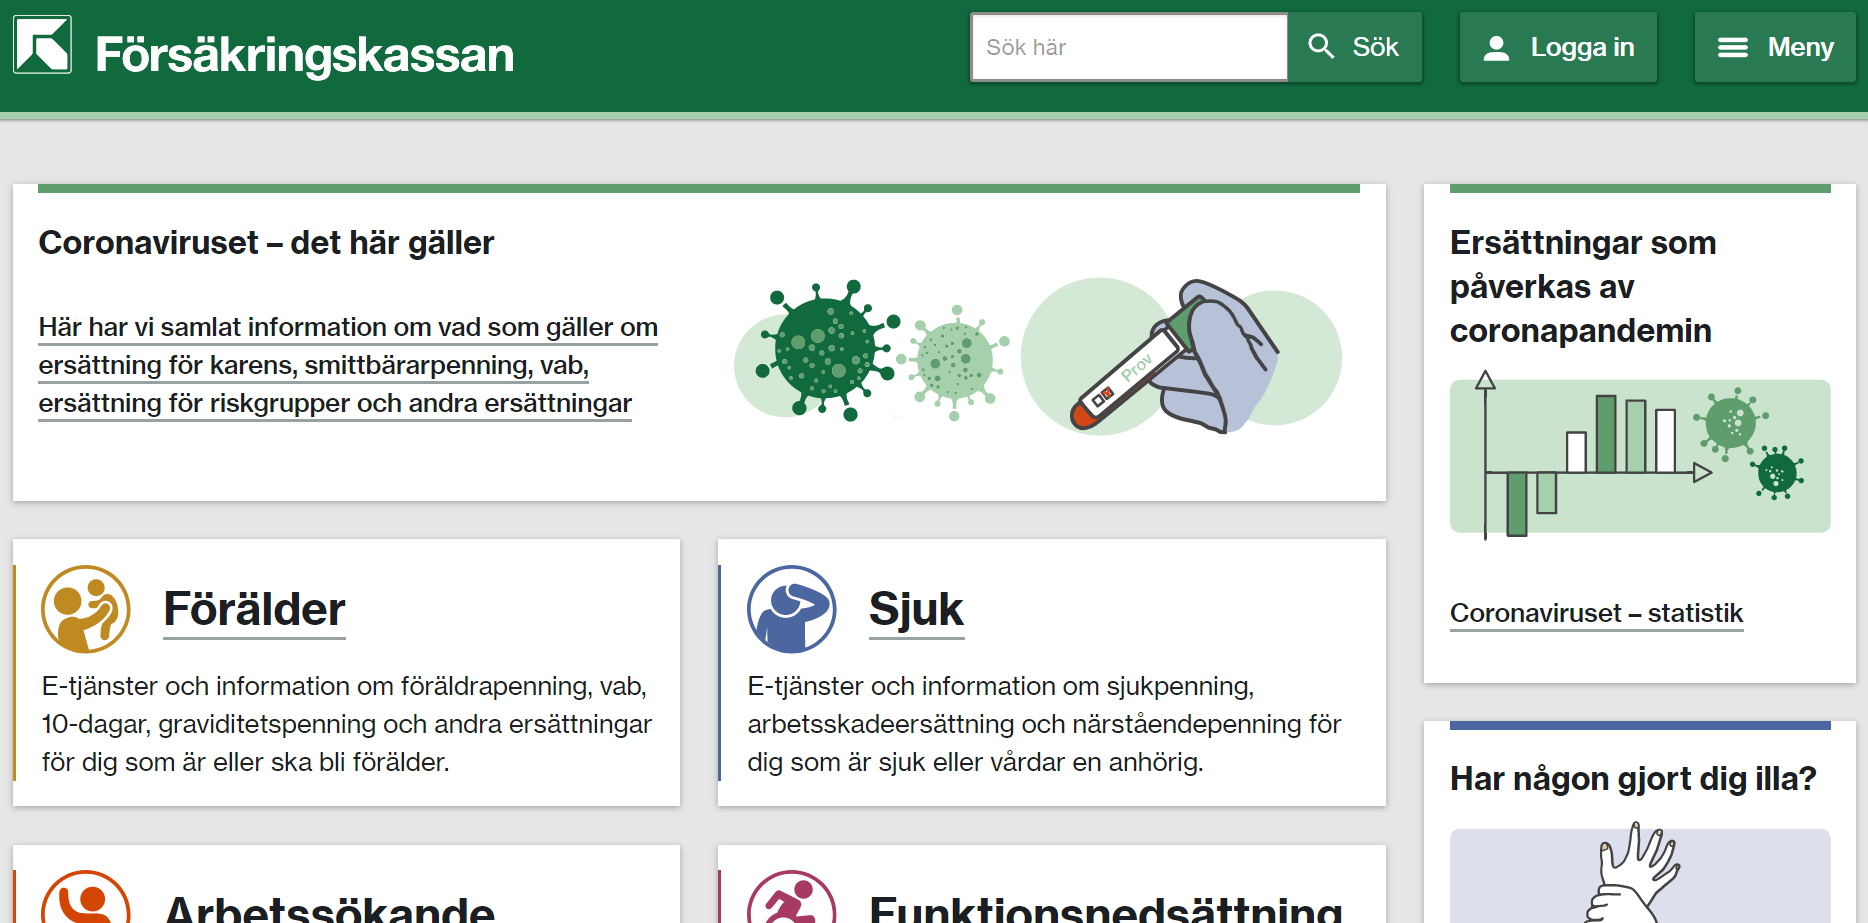
\includegraphics[width=15cm,height=15cm,keepaspectratio]{figure/seq/socity site of sweed.PNG}
  \caption{Site officiel de la sécurité sociale de Suède}
\end{figure}
\\\\

\textbf{La sécurité sociale en États-Unis d'Amérique} [2] : Aux États-Unis, la sécurité sociale est le terme couramment utilisé pour le programme fédéral d’assurance vieillesse, survivants et invalidité (OASDI) et est administré par l’Administration de la sécurité sociale. La première Loi sur la sécurité sociale a été promulguée par Franklin D. Roosevelt en 1935 et la version actuelle de la Loi, telle que modifiée, englobe plusieurs programmes d’aide sociale et d’assurance sociale.\\

\begin{figure}[!h]
  \centering

\includegraphics[width=15cm,height=15cm,keepaspectratio]{figure/socity site of america.PNG}
  \caption{Site officiel de la sécurité sociale des États-Unis}
\end{figure}


\newpage

% \chapter{Analyse et Conception}
\chapter{Analyse des besoins}

\section{Introduction}
% Ce chapitre présente la partie conception qui sert à réaliser des différents types de
% diagramme qui modélise les différentes parties du projet afin de mieux comprendre l'application.


Dans ce chapitre , nous allons montrer les fonctionnalités de chaque acteur
avant de pouvoir passer à la conception de notre projet.
 \section{ Les besoins fonctionnels}
  \subsection{ Présentation des acteurs}
Premièrement, les acteurs sont des entités externes par rapport à un système modélisé et qui intéragissent avec ce système. Identifier les acteurs intervenant peut en fait représenter une véritable problématique. Pour nous aider à mieux les identifier, voici
quelques questions qui nous permettront plus facilement d'identifier les acteurs de notre système :
\vspace{0.2cm}
% \begin{enumerate}
% \item Third level, enumerate, first item
% \item Third level, enumerate, second item
% \end{enumerate}
\begin{enumerate}
\item Quels sont les utilisateurs qui ont besoin d'un système pour réaliser le
travail ?

\item  Quels sont les utilisateurs qui vont effectuer les actions principales du
système ?

\item Quels sont les utilisateurs qui vont exécuter les fonctions principales
du système (maintenance et administration) ?

\item Est-ce que le système interagit avec le matériel ou d'autres logiciels ?
\vspace{0.2cm}
\end{enumerate}
En se basant uniquement sur ces quatre dernières questions, nous pouvons
facilement identifier nos acteurs.
Pour notre système ,bien évidemment notre application web, nous avons
quatre acteurs :\\
\begin{itemize}
\item[$\bullet$] Le citoyen\\
\item[$\bullet$] L'empolyé\\
\item[$\bullet$] L'administrateur
\end{itemize}

\newpage
 \subsection{ Identification des fonctionnalités par acteur}
 Nous présenterons dans ce qui suit la fonction de chacun de nos utilisateurs :\\\\
\large{\textbf{      Fonctionnalité du citoyen : }}
 \newpage
 \section{ Les besoins non fonctionnels}
\begin{itemize}


\item[$\bullet$] \textbf{L'utilisation :}  L'application doit être facile à utiliser, être adaptée aux différents citoyens,  dont le but général est de les satisfaire.\\


\item[$\bullet$]\textbf{L’extensibilité :} l’application devra être extensible, c’est-à-dire qu’il pourra y avoir une possibilité d’ajouter ou de modifier des nouvelles fonctionnalités. \\

\item[$\bullet$] \textbf{La performance : }: Est l'une des premières exigences d'une application
web, et surtout les applications destinées au grand public. Ce dernier juge souvent
la performance par le temps de réponse de l'application, donc notre application doit
répondre rapidement aux actions des utilisateurs, et s'il y a un traitement qui peut
prendre de temps, il vaut mieux l'exécuter en arrière-plan.
\\

\item[$\bullet$] \textbf{L’interface :} Avoir une interface de bon niveau surtout que l’utilisation des Smartphones et des tablettes imposées que l’interface soit adaptative. \\




% \item[$\bullet$] \textbf{La convivialité :} L’application doit être simple et facile à manipuler par les utilisateurs.

\end{itemize}
% % Ce diagramme est classé comme un modèle statique du système, il sert à réaliser une
% % modélisation des relations entre les classes du système orienté objet.

% % \begin{figure}[!h]
% %   \centering
% %   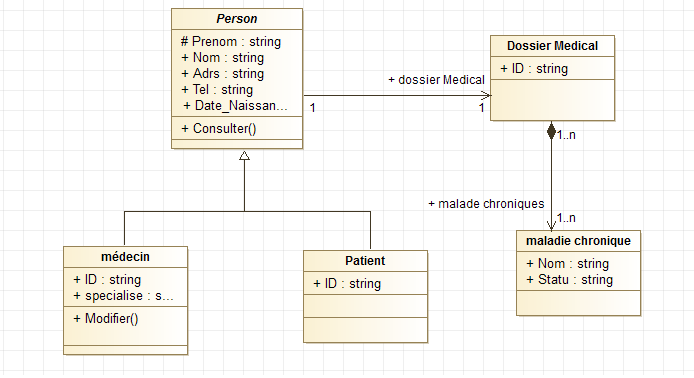
\includegraphics[width=15cm,height=15cm,keepaspectratio]{figure/seq/fig4.png}
% %   \caption{Diagramme de classes}
% % \end{figure}

% % La figure  présente le diagramme de classes de notre projet :

% % \begin{description}

% %   \item[Person : ] c’est la classe qui contient les informations generales sur les utilisateurs .
% %   \item[Patient : ]c’est une classe qui hérite de la classe  Person  et qui dispose des attributs et des opérations supplémentaires concernant le patient.
% %   \item[Medécin : ] c’est une classe qui hérite de la classe  Person  et qui dispose des attributs et des opérations supplémentaires concernant le médecin.
% %   \item[Dossier Medical : ] c’est la classe qui contient les informations médicales pour chaque patient  .
% %   \item[Maladie Chronique : ] c’est la classe qui contient la statut et les information de chaqun des maladies chroniques qui est dans le dossier medical  .

% % \end{description}

% \section{Diagramme de cas d'utilisation }
% Ce diagramme  capture le comportement d'un système,
% d'un sous-système, d'une classe ou d'un composant, il représente une interaction entre un
% utilisateur (humain ou machine) et un système, les utilisateurs sont appelés acteurs ils
% interagissent avec les cas d'utilisation.\\
% \begin{figure}[!h]
%   \centering
% 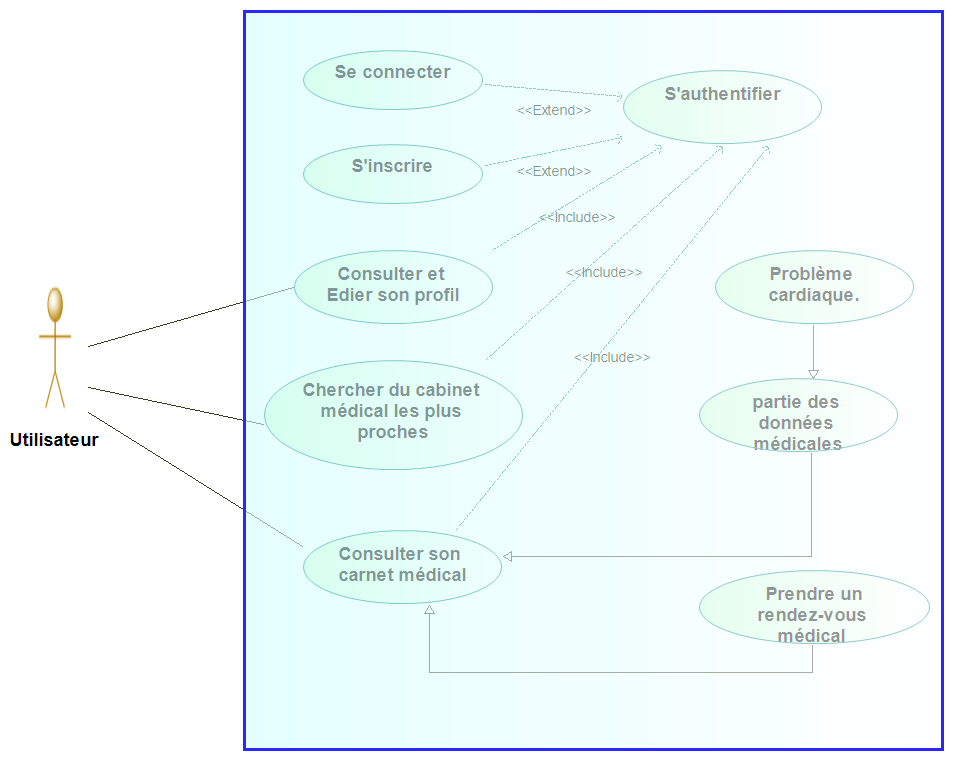
\includegraphics[width=15cm,height=15cm,keepaspectratio]{figure/fg9.png}
%   \caption{ Diagramme de cas d'utilisation}
% \end{figure}

% Le  diagramme  de cas  d'utilisation  ci-dessus  nous  montre  l'interaction  entre  l'utilisateur  et l'application , l'utilisateur doit s'authentifier pour  accéder à une page d'accueil .
% \newpage
% \section{Les diagrammes de séquences}
% Les diagrammes de séquence peuvent servir à illustrer les cas d’utilisations décrits dans la
% partie précédente . Ils permettent de représenter la succession chronologique des opérations
% réalisées par un acteur et qui font passer d’un objet à un autre pour représenter un scénario.
% Dans cette partie, nous allons décrire les scénarios les plus importants ainsi que leurs
% représentations par les diagrammes de séquence

% \subsection{Cas d’utilisation « Connection »  }
% \begin{figure}[!h]
%   \centering
% 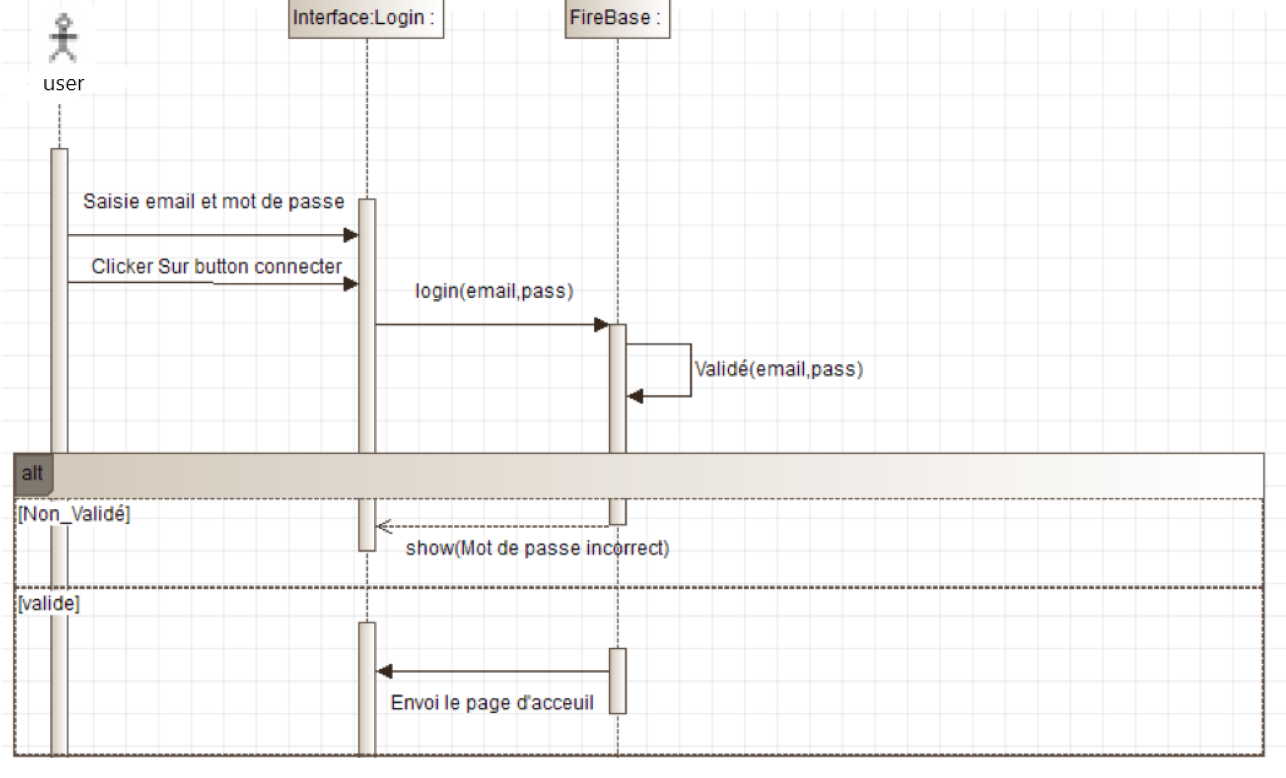
\includegraphics[width=15cm,height=20cm,keepaspectratio]{figure/seq/fig1.png}
%   \caption{Diagramme de séquence du cas d'utilisation "s'authentifier"}
% \end{figure}

% La figure  représente les différentes séquences qui se produisent lorsqu’un utilisateur
% appuie sur le bouton de connexion (Sing in) de l’interface d’authentification, le système  va
% tout d’abord tester s’il y a un champ vide ou invalide, après il va demander au serveur de Firebase de
% vérifier les informations d’authentification .
% \newpage
% \subsection{Cas d’utilisation « Inscription »  }
% \begin{figure}[!h]
%   \centering
% 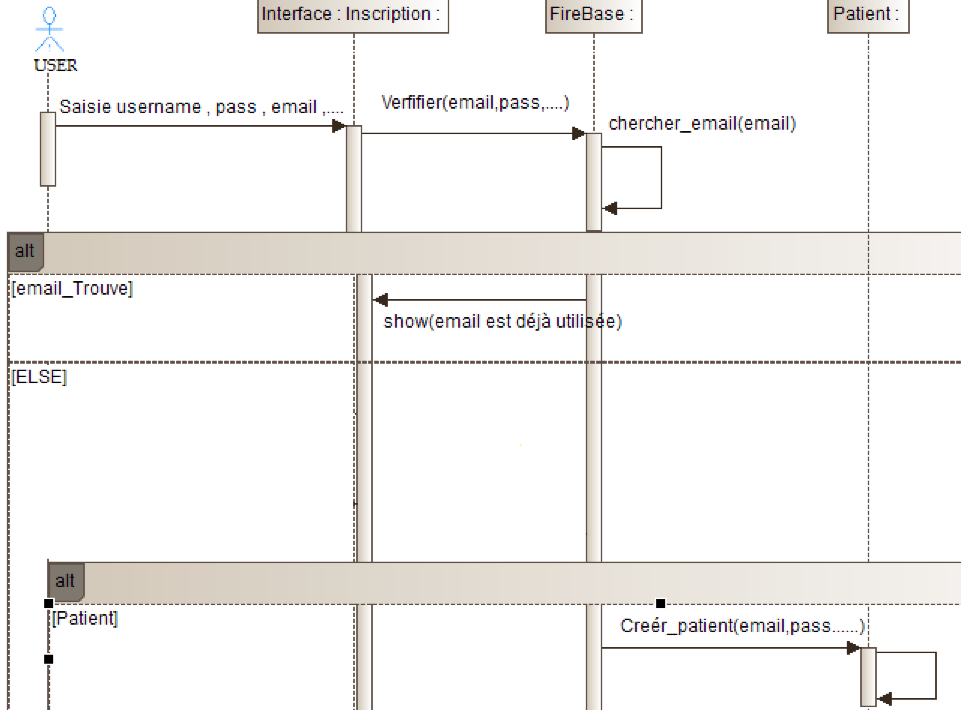
\includegraphics[width=15cm,height=20cm,keepaspectratio]{figure/seq/fig3.png}
%   \caption{Diagramme de séquence du cas d'utilisation "Inscription"}
% \end{figure}

% La figure  représente les différentes séquences qui se produisent lorsqu’un utilisateur
% appuie sur le bouton d'inscrir (Sing up) , le système  va
% tout d’abord tester s’il y a un champ vide ou invalide et si gmail a été déjà utilisé  après il va demander au serveur de Firebase de
% vérifier les informations d’inscrir puis creer un compte dans la base de donnée .
% \newpage
% \subsection{Cas d’utilisation « Password reset  »  }
% \begin{figure}[!h]
%   \centering
% 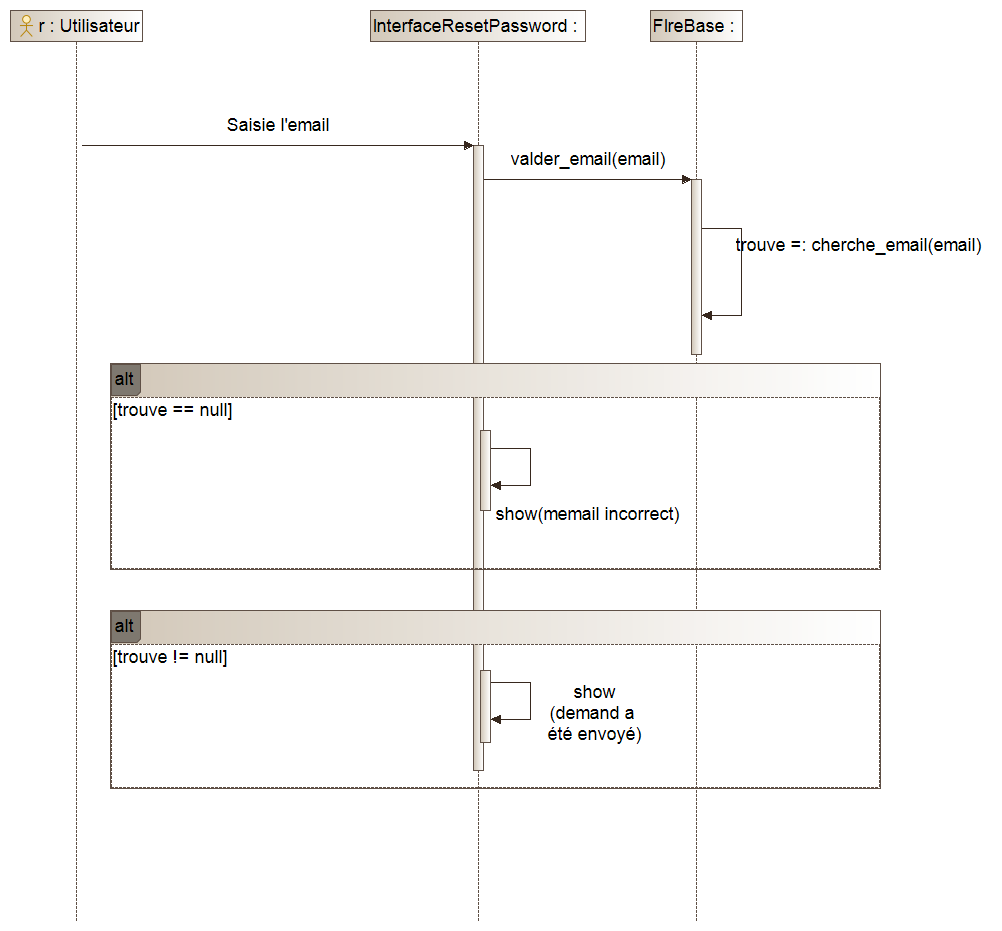
\includegraphics[width=15cm,height=20cm,keepaspectratio]{figure/seq/fig2.png} \\
%   \caption{Diagramme de séquence du cas d'utilisation "password reset "}
% \end{figure}

% La figure  représente les différentes étapes qui se produisent lorsqu’un utilisateur a oublué  son email, donc il faut à l'utilisateur  a envoyé son gmail pour reçois leur mot de passe à leur gmail.


% \section*{Conclusion }
% Ce chapitre a présenté la conception de notre application mobile. Nous
% avons détaillé la conception de notre application à travers  diagrammes de
% classe , diagrammes de cas d'utilisation ,  ainsi que Les diagrammes de séquences associées afin que la phase
% réalisation et la mise en place de l’application mobile soit plus souple et
% plus aisée. Cette conception a été faite en UML. \\
% Dans le chapitre suivant, nous  avons donné un aperçu sur l'ensemble des outils utilisés realiser cet application.
% % ,
% % framework et langages utilisés pour 

\newpage

\chapter{Realisation}

\section*{Introduction}
Pour pouvoir mener à bien notre application mobile, il est nécessaire de choisir des technologies permettant de simplifier sa réalisation. Pour cela, et après avoir élaboré une conception détaillée des cas d’utilisation, les diagrammes de séquence, ainsi que le diagramme de classe complet dans le chapitre précédent, nous abordons la partie réalisation dans ce qui suit.

\section{Environnement de développement }
\subsection{TypeScript}
\begin{figure}[!h]
  \centering

\includegraphics[width=3cm,height=3cm,keepaspectratio]{figure/fig2.PNG}
  \caption{icon TypeScript}
\end{figure}


TypeScript est un langage open-source qui s’appuie sur JavaScript, l’un des outils les plus utilisés au monde, en ajoutant des définitions de types statiques.\\

Les types fournissent un moyen de décrire la forme d’un objet, fournissant une meilleure documentation et permettant à TypeScript de valider que votre code fonctionne correctement.


% \subsection{React Native}

% \begin{figure}[!h]
%   \centering
%   
\includegraphics[width=4cm,height=4cm,keepaspectratio]{figure/fig7.png}
%   \caption{Icon du XML }
% \end{figure}

% Un framework créé par Facebook à la suite d'un Hackaton en 2015 et une librairie Javascript développée deux ans auparavant par un ingénieur Facebook (Jordan Walke). React Native sont pratiquement identiques à ceux de React, à la différence que React Native ne manipule pas le DOM via le DOM virtuel. Il s'exécute dans un processus en arrière - plan (qui interprète le code JavaScript écrit par les développeurs) ,React Native n'utilise pas HTML. Au lieu de cela, les messages du thread JavaScript sont utilisés pour manipuler des vues natives.



% \section{Langages de programmation android }
% Il est indispensable de bien connaître Java avant de pouvoir développer pour Android, mais la plupart des développeurs utilisent également XML. Ces deux langages sont en effet recommandés par Google pour la création des applications Android.

% \newpage
\subsection{React Native}

\begin{figure}[H]
  \centering
 
\includegraphics[width=3cm,height=3cm,keepaspectratio]{figure/fig7.png}
  \caption{Icon du React Native }
\end{figure}

 Un framework créé par Facebook à la suite d'un Hackaton en 2015 et une librairie Javascript développée deux ans auparavant par un ingénieur Facebook (Jordan Walke). React Native sont pratiquement identiques à ceux de React, à la différence que React Native ne manipule pas le DOM via le DOM virtuel. Il s'exécute dans un processus en arrière - plan (qui interprète le code JavaScript écrit par les développeurs) ,React Native n'utilise pas HTML. Au lieu de cela, les messages du thread JavaScript sont utilisés pour manipuler des vues natives.


\subsection{Base de données : FireBase}

\begin{figure}[H]
  \centering
 
\includegraphics[width=3cm,height=3cm,keepaspectratio]{figure/fig2.png}
  \caption{Icon du Firebase }
\end{figure}

Firebase est un ensemble de services d'hébergement pour n'importe quel type d'application (Android, iOS, Javascript, Node.js, Java, Unity, PHP, C++ ...).\\ Il propose d'héberger en NoSQL et en temps réel des bases de données, du contenu, de l'authentification sociale (Google, Facebook, Twitter et Github), et des notifications, ou encore des services, tel que par exemple un serveur de communication temps réel.
\newpage
\subsection{Les services de Firebase}
Les services de Firebase sont : \\
\begin{figure}[H]
  \centering
 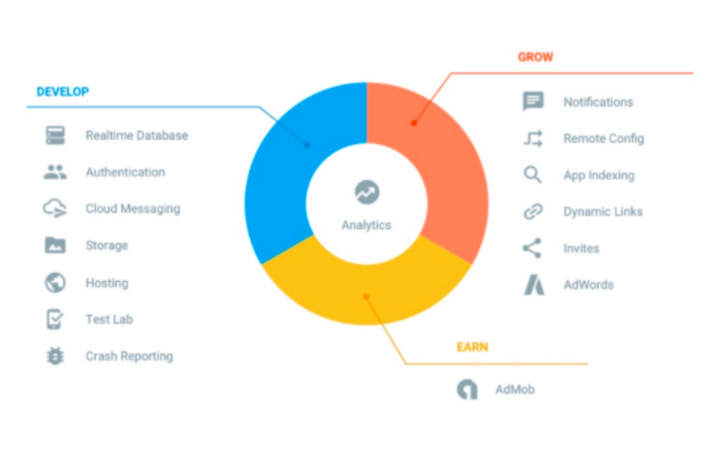
\includegraphics[width=11cm,height=11cm,keepaspectratio]{figure/fig3.png}
  \caption{Icon du sersvices de FireBase }
\end{figure}
\\
\begin{itemize}
\item Créez des applications rapidement, sans gérer l'infrastructure\\
\item Soutenu par Google, approuvé par les meilleures applications\\
\item Une plateforme, avec des produits qui fonctionnent mieux ensemble\\

\end{itemize}

% \subsection{Firebase Realtime Database}
% Firebase Realtime Database est une base de données NoSQL hébergée dans le cloud qui nous permet de stocker et de synchroniser des données entre les utilisateurs en temps réel.
% \\La synchronisation en temps réel permet à les utilisateurs d'accéder facilement à leurs données depuis n'importe quel appareil, que ce soit sur le Web ou sur un appareil mobile. La base de données en temps réel permet également à les utilisateurs de collaborer les uns avec les autres.

% Un autre gros avantage de Realtime Database est qu'elle est livrée avec des SDK mobiles et Web, nous permettant de créer vos applications sans avoir besoin de serveurs.

% \begin{figure}[h]
%   \centering

% 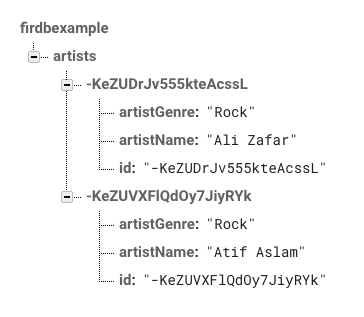
\includegraphics[width=10cm,height=10cm,keepaspectratio]{figure/fg4.png}
% \caption{example d'une base de donneés NoSQL  }
% \end{figure}
% Lorsque vos utilisateurs sont hors ligne, les SDK de base de données en temps réel utilisent le cache local sur l'appareil pour servir et stocker les modifications.\\
%  Lorsque l'appareil est en ligne, les données locales sont automatiquement synchronisées.

% \subsection{Firebase Authentication}
% \begin{figure}[h]
%   \centering
% 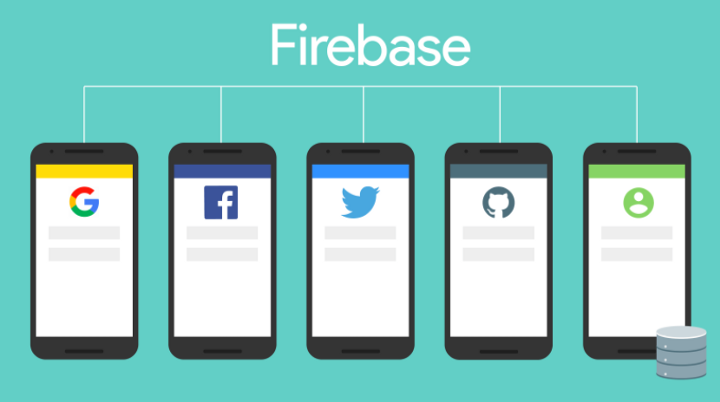
\includegraphics[width=7cm,height=5cm,keepaspectratio]{figure/fg5.png}
% \caption{Firebase Authentication}
% \end{figure}



% Firebase Authentication fournit des services backend, des SDK faciles à utiliser et des bibliothèques d'interfaces utilisateur prêtes à l'emploi pour authentifier les utilisateurs de votre application.
% \\Vous pouvez authentifier les utilisateurs de votre application à l'aide des méthodes suivantes:
% \begin{itemize}
%   \item Email et mot de passe
%   \item Numéro de téléphone
%   \item Google
%   \item Facebook
%   \item Twitter
%   \item etc !
% \end{itemize}

% L'utilisation de Firebase Authentication facilite la création de systèmes d'authentification sécurisés, tout en améliorant l'expérience de connexion et d'intégration pour les utilisateurs finaux.

% \section{La gestion du base de données}
% \subsection{Intégrez Firebase dans une application Android}

% Les projets Firebase sont des projets Google Cloud Platform qui utilisent les services Firebase et présentent les caractéristiques suivantes :

% La facturation et les autorisations relatives aux projets sont partagées entre les différentes consoles.
% Les projets qui apparaissent dans la console Firebase apparaissent également dans les consoles API Google et Google Cloud Platform.
% Lorsqu’un projet est supprimé, il est supprimé sur toutes les consoles.

% 1 – En premier lieu, si vous n’avez aucun compte Gmail, la première étape sera d’en créer un.

% 2 – Connectez-vous sur la Console Google Firebase : https://console.firebase.google.com/

% 3 – Cliquez en haut à droite sur « accéder à la console »
% \begin{figure}[h]
%   \centering
%   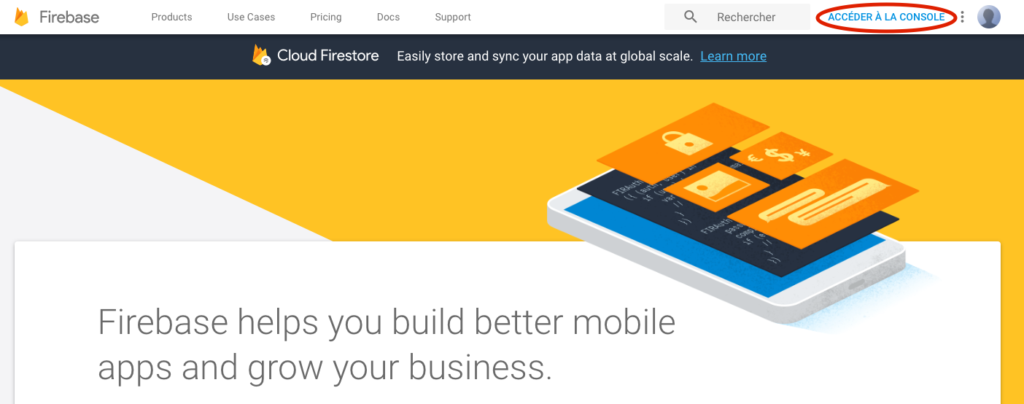
\includegraphics[width=15cm,height=10cm,keepaspectratio]{figure/fig14.png} \\
%   \caption{Interface de la page de Firebase }
% \end{figure}



% 4 – Sélectionnez le projet ou bien ajoutez un projet

% Pour ajouter un projet : Cliquer sur « ajouter un projet » cette page (photo ci-dessous) s’affiche. Il vous suffira de remplir de nom du projet et sélectionner le pays avec la liste déroulante puis cliquer sur « créer un projet »

% \begin{figure}[H]
%   \centering
%   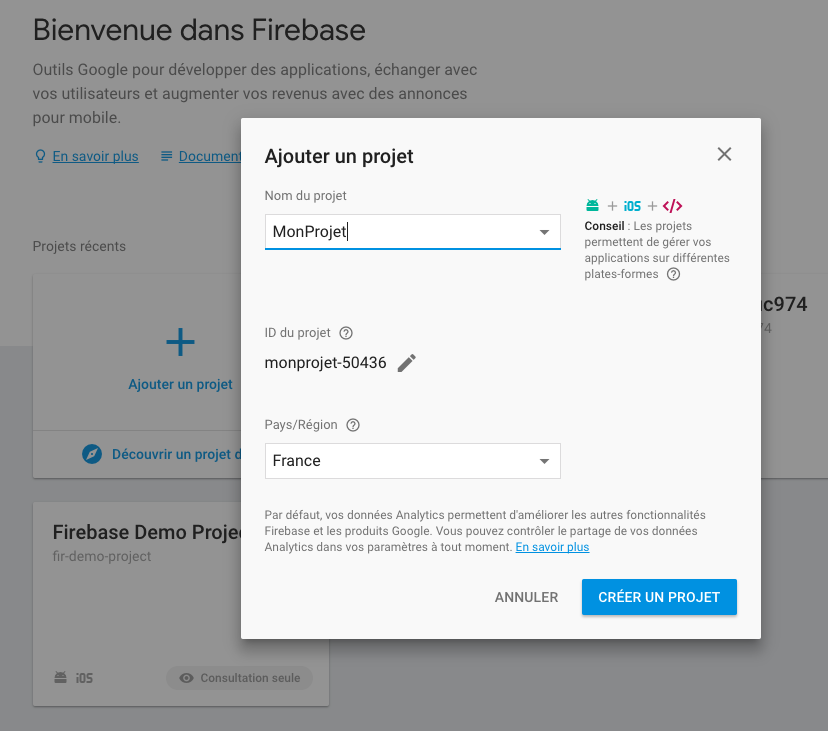
\includegraphics[width=15cm,height=10cm,keepaspectratio]{figure/fig15.png} 
% \end{figure}

% 5 – Une fois sur le projet, une nouvelle page s’affiche. Cliquez sur l’icône « Ajouter Firebase à votre application Android » (entouré en rouge sur la photo) \\

% 6 – Remplissez le « nom de package de votre application Android ». Pour cela, il faudra le demander au développeur, puis cliquez sur « Enregistrer l’application »
% \begin{center}
%   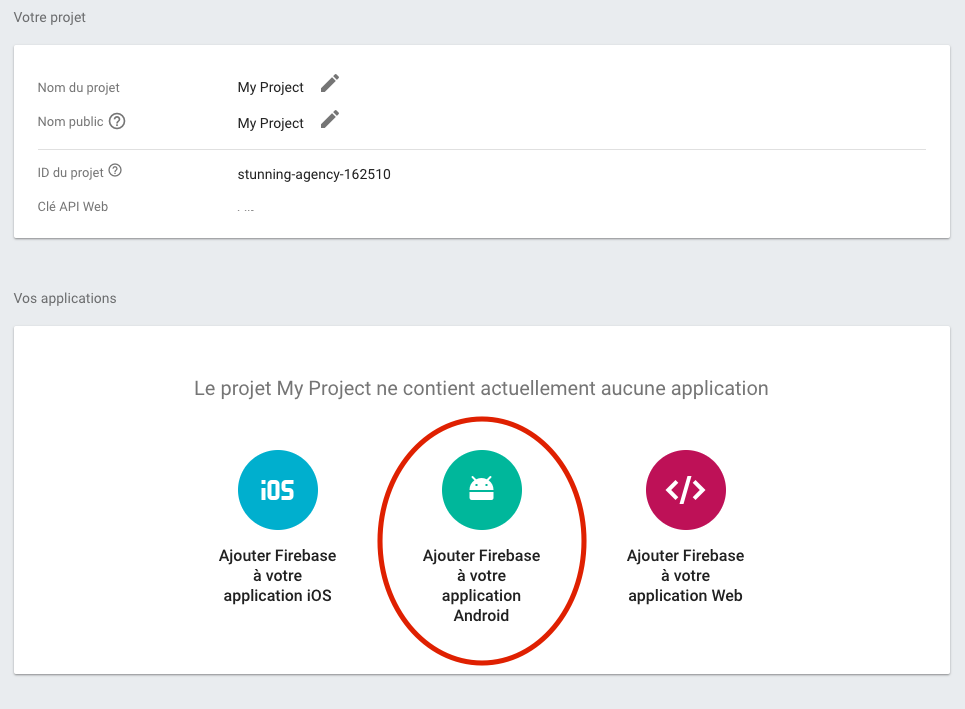
\includegraphics[width=10cm,height=10cm,keepaspectratio]{figure/fig16.png} \\
%   \end{center}


%  7 – Téléchargez le fichier « google-service-json » (gardez le fichier pour l’intégrer dans l’application) grâce au bouton et cliquez sur « Continuer »
%  \begin{center}
%   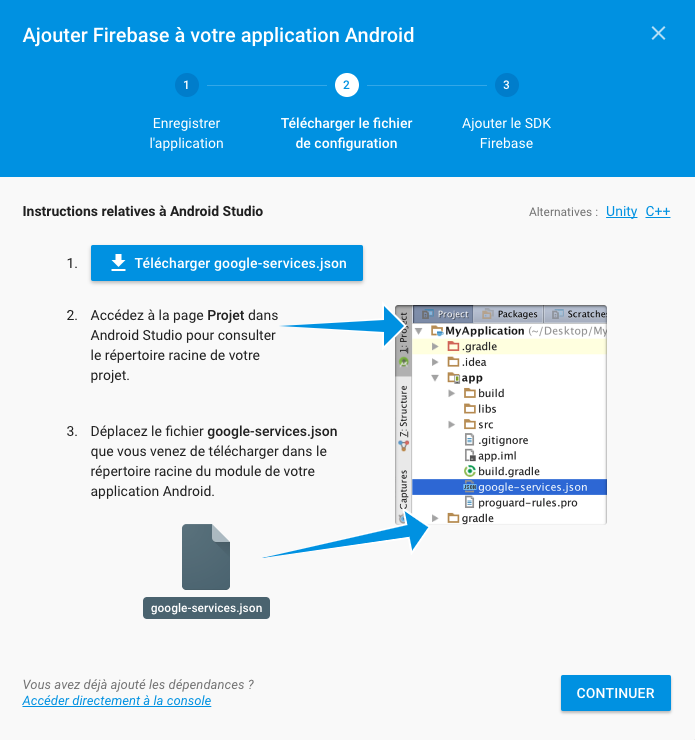
\includegraphics[width=15cm,height=10cm,keepaspectratio]{figure/fig18.png} \\
%   \end{center}

% \subsection{Structure de données}
% Sur Firebase, il existe deux types de bases de données : Firebase Realtime Database et Firebase Firestore. Ces dernières sont des bases de données dites "NoSQL" . \\
% \begin{figure}[H]
%   \centering
% 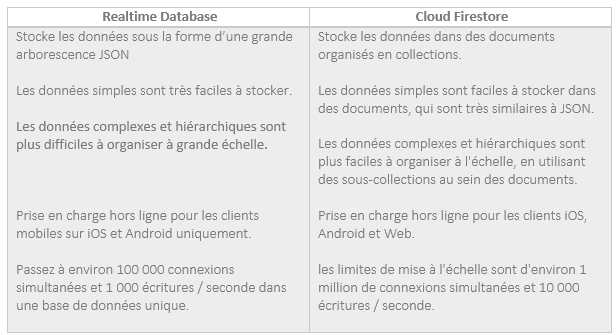
\includegraphics[width=13cm,height=15cm,keepaspectratio]{figure/fig19.png}
%   \caption{firebase realtime database vs firestore}
% \end{figure}

% \subsection{Lire et écrire des données FireBase  }
% Les données Firebase sont écrites dans une référence FirebaseDatabase et récupérées en attachant un écouteur asynchrone à la référence. L'écouteur est déclenché une fois pour l'état initial des données et à chaque fois que les données changent .
% Pour lire ou écrire des données de la base de données, vous avez besoin d'une instance de DatabaseReference:
% \begin{center}
%     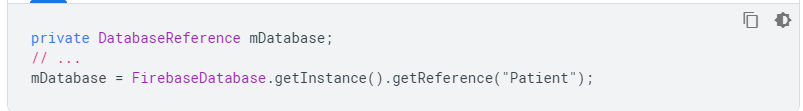
\includegraphics[width=15cm,keepaspectratio]{figure/fig21.png} \\
% \end{center}

% pour ajouter ou modifier un objet,valeur Doit être utilisé setValue ():
% \begin{center}
%     
\includegraphics[width=15cm,keepaspectratio]{figure/fig22.png} \\
% \end{center}

% Pour obtenir les données,il doit définir un écouteur pour la référence. \\
% Il existe essentiellement deux types d'écouteurs que vous pouvez attacher, l'un est ValueEventListener et l'autre est ChildEventListener . Pour tout changement de données sous le nœud auquel nous avons des références et des écouteurs ajoutés, les écouteurs d'événement de valeur renvoient la structure JSON complète et l'écouteur d'événement enfant retourne un enfant spécifique où la modification s'est produite. Les deux sont utiles à leur manière. Pour extraire les données de Firebase, nous pouvons ajouter un ou plusieurs écouteurs à une référence de base de données firebase .
% Voici un exemple de code (code explicatif après code):
%     \begin{center}
%     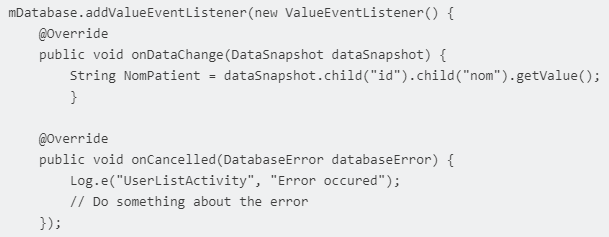
\includegraphics[width=15cm,keepaspectratio]{figure/fig23.png} \\
% \end{center}



\section*{Conclusion }
Ce chapitre contient l'ensemble des outils, framework et languages utilisés pour créer notre application.
Par la suite, nous allons à la phase de la description des interfaces graphiques de l'application. 

\newpage

\chapter{Description Les interfaces de Réalisation }


\section*{introduction}

Nous allons introduire dans ce chapitre les interfaces graphiques que nous avons dû
à réaliser, nous vous présentons ces interfaces sous formes captures d'écran, ainsi que des
explications montrant le déroulement de notre application :




\section{Connection:}
Pour accéder à notre application l'utilisateur doit se connecter ou creér un compte . Comme toutes les applications qui comportent des informations personelles, la sécurité d'accès est nécessaire. La figure ci-après donne l'interface à travers laquelle l'utilisateur s'identifie. Il saisit son E-mail et son mot de passe puis l'application  vérifie si cet utilisateur existe en base donnée ou pas.

\begin{figure}[H]
  \centering
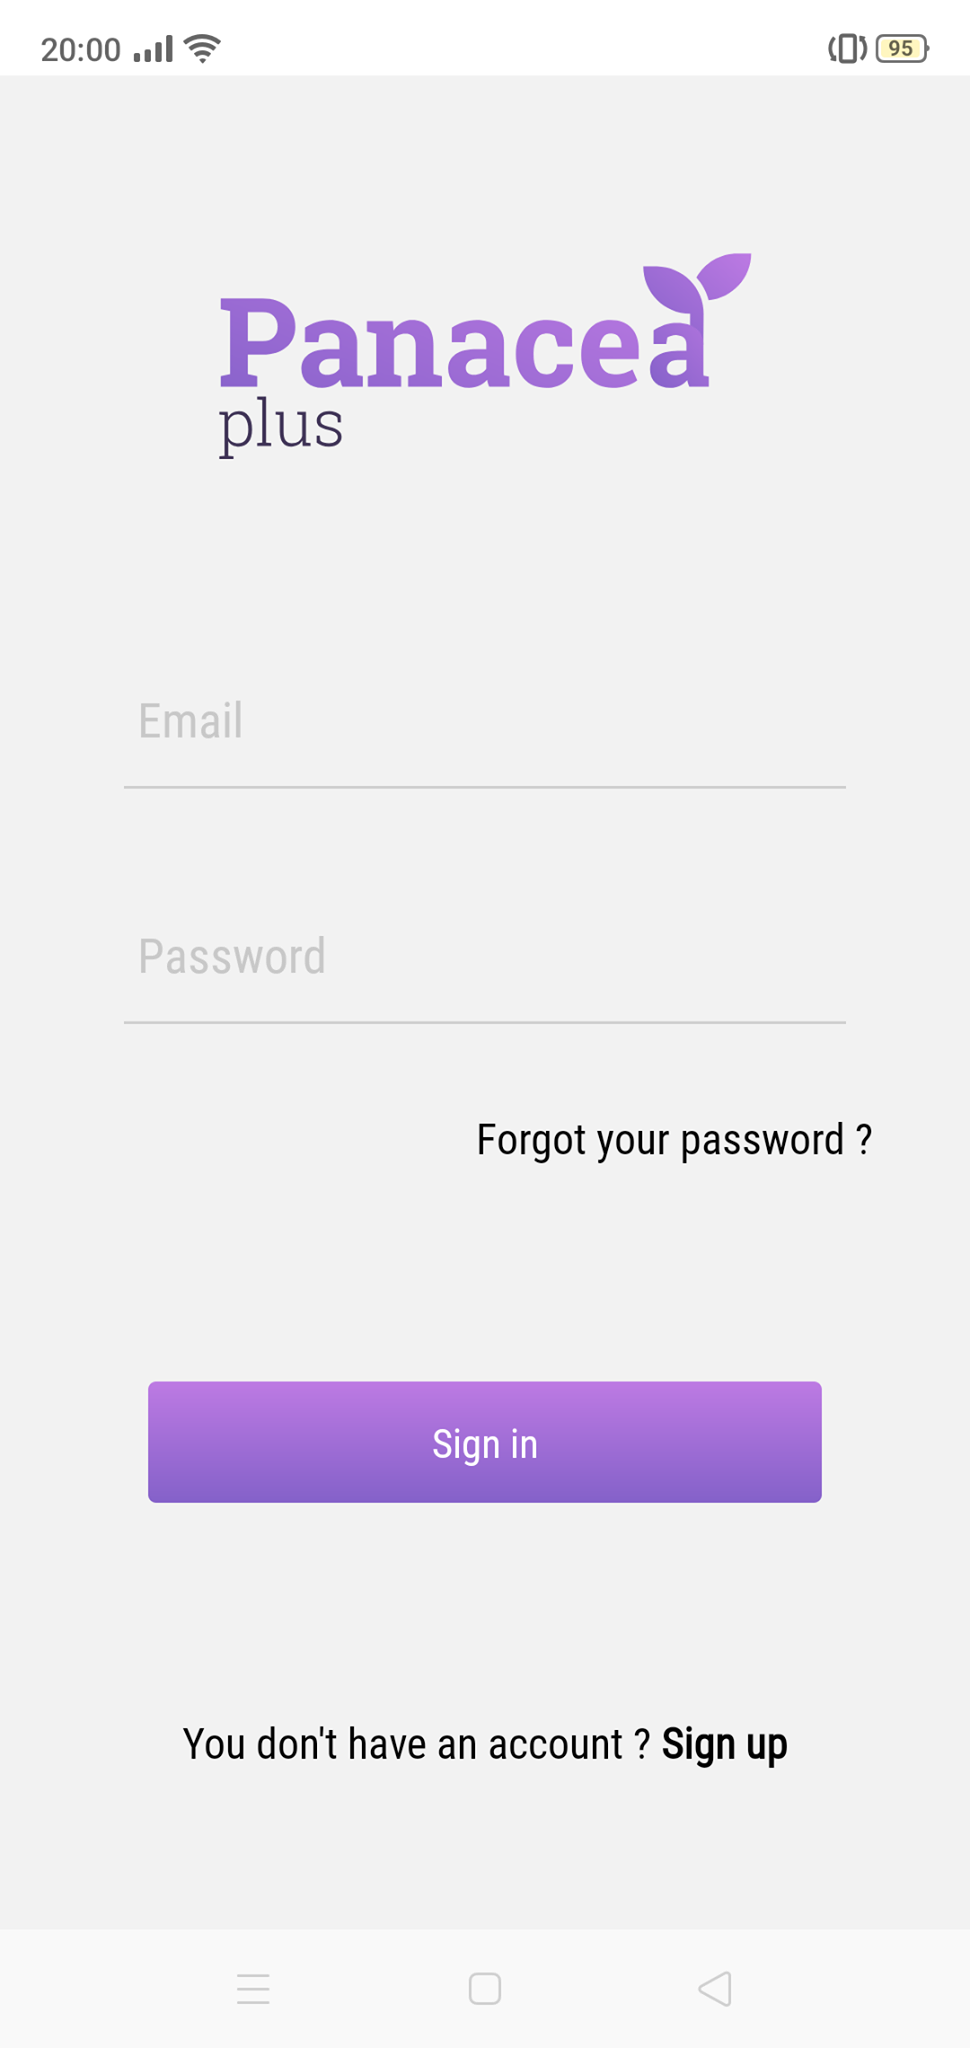
\includegraphics[width=11cm,height=11cm,keepaspectratio]{Application/connecter.png} 
\caption{Interface de se connecter}
\end{figure}

Le message d'erreur sera afficher dans le cas où les information n'existent pas dans notre base de données ou dans le cas d'abscense d'accès à l'internet.
\begin{figure}[H]
  \centering
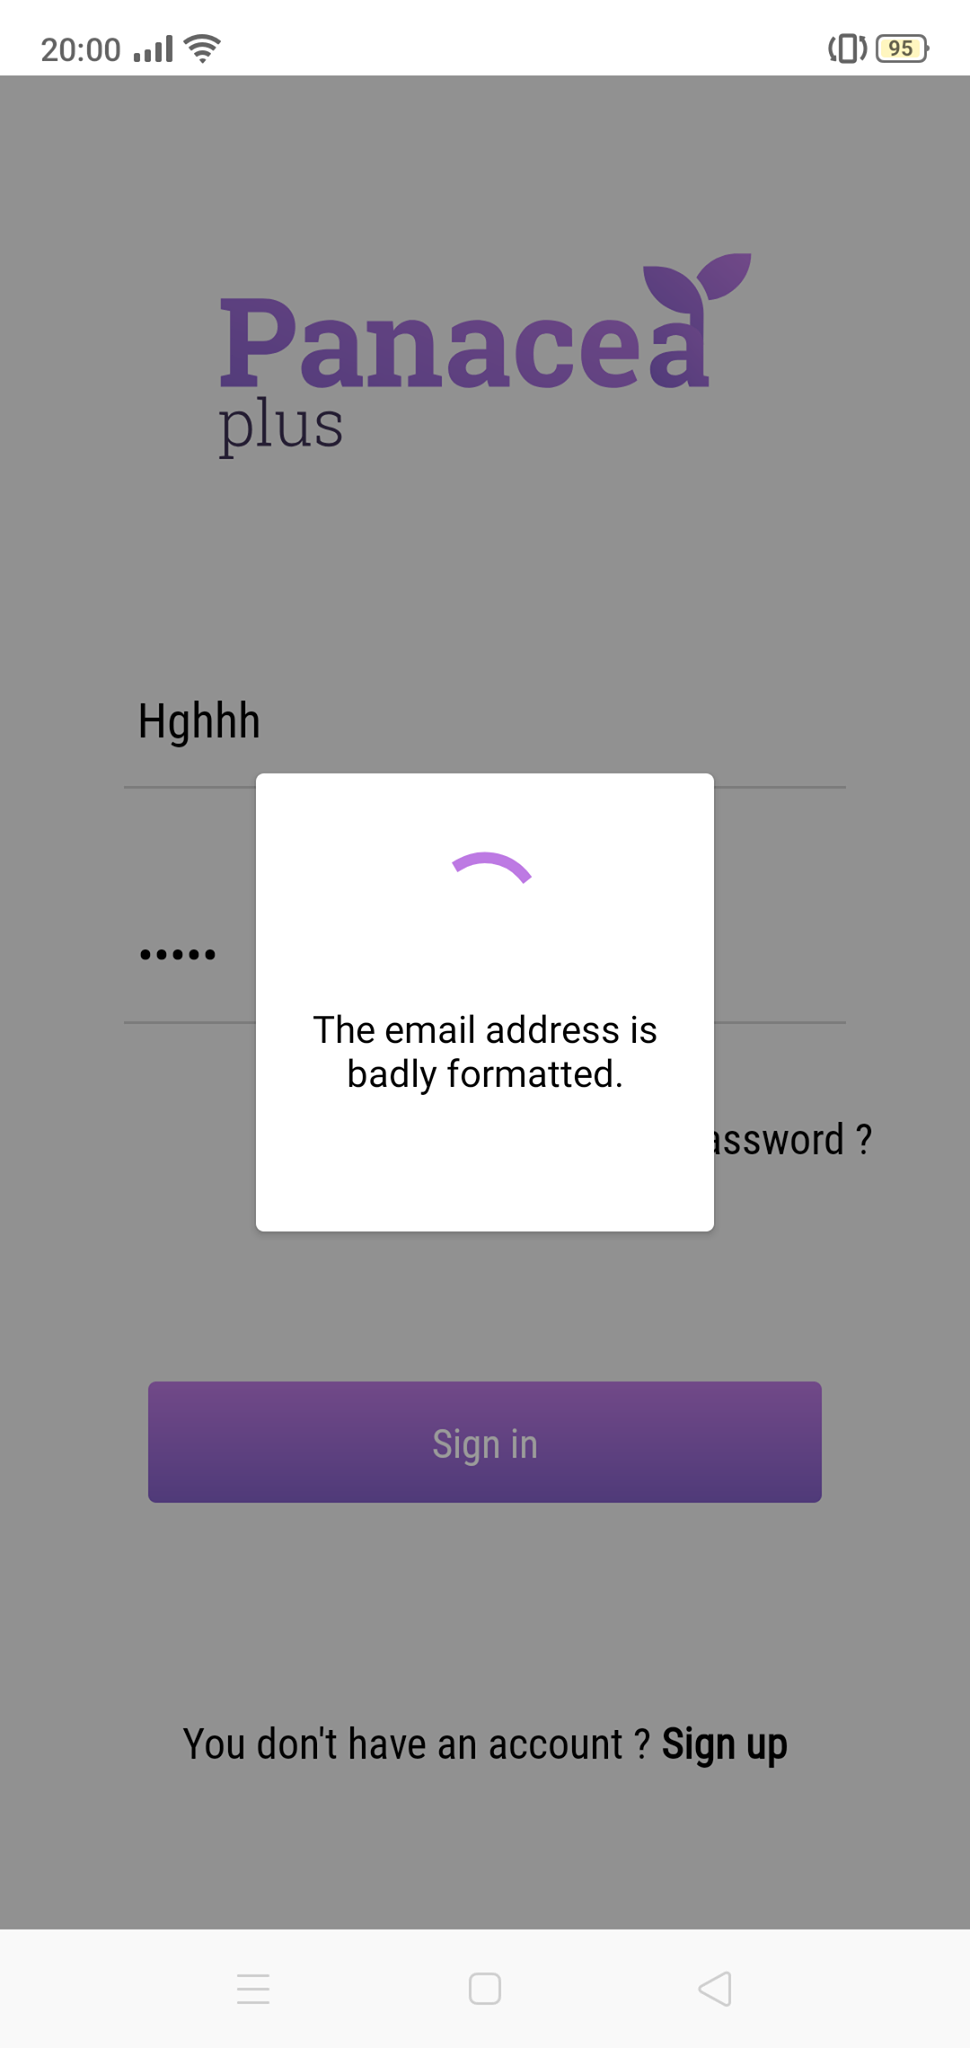
\includegraphics[width=8cm,height=8cm,keepaspectratio]{Application/er.png} 
\caption{Interface de connection en cas d’erreur}
\end{figure}

Une fois les données sont valides, l'utilisateur peut accéder à la page d'accueil.
% Les utilisateurs principaux de l'application sont les médecins et les patients , chaque utilisateur a sa propre interface d'accueil.
\section{Inscription}

Pour créer un nouveau compte il faut d'abord que l’utilisateur  appuie sur Sing up (première interface ) après l'application il va dirige l'utilisateur vers l'interface de l'inscription
% choisie s'il est un médecin ou un patient puis il va être diriger vers l'interface suivant pour saisie ses informations :
% \begin{figure}[H]
%   \centering
%   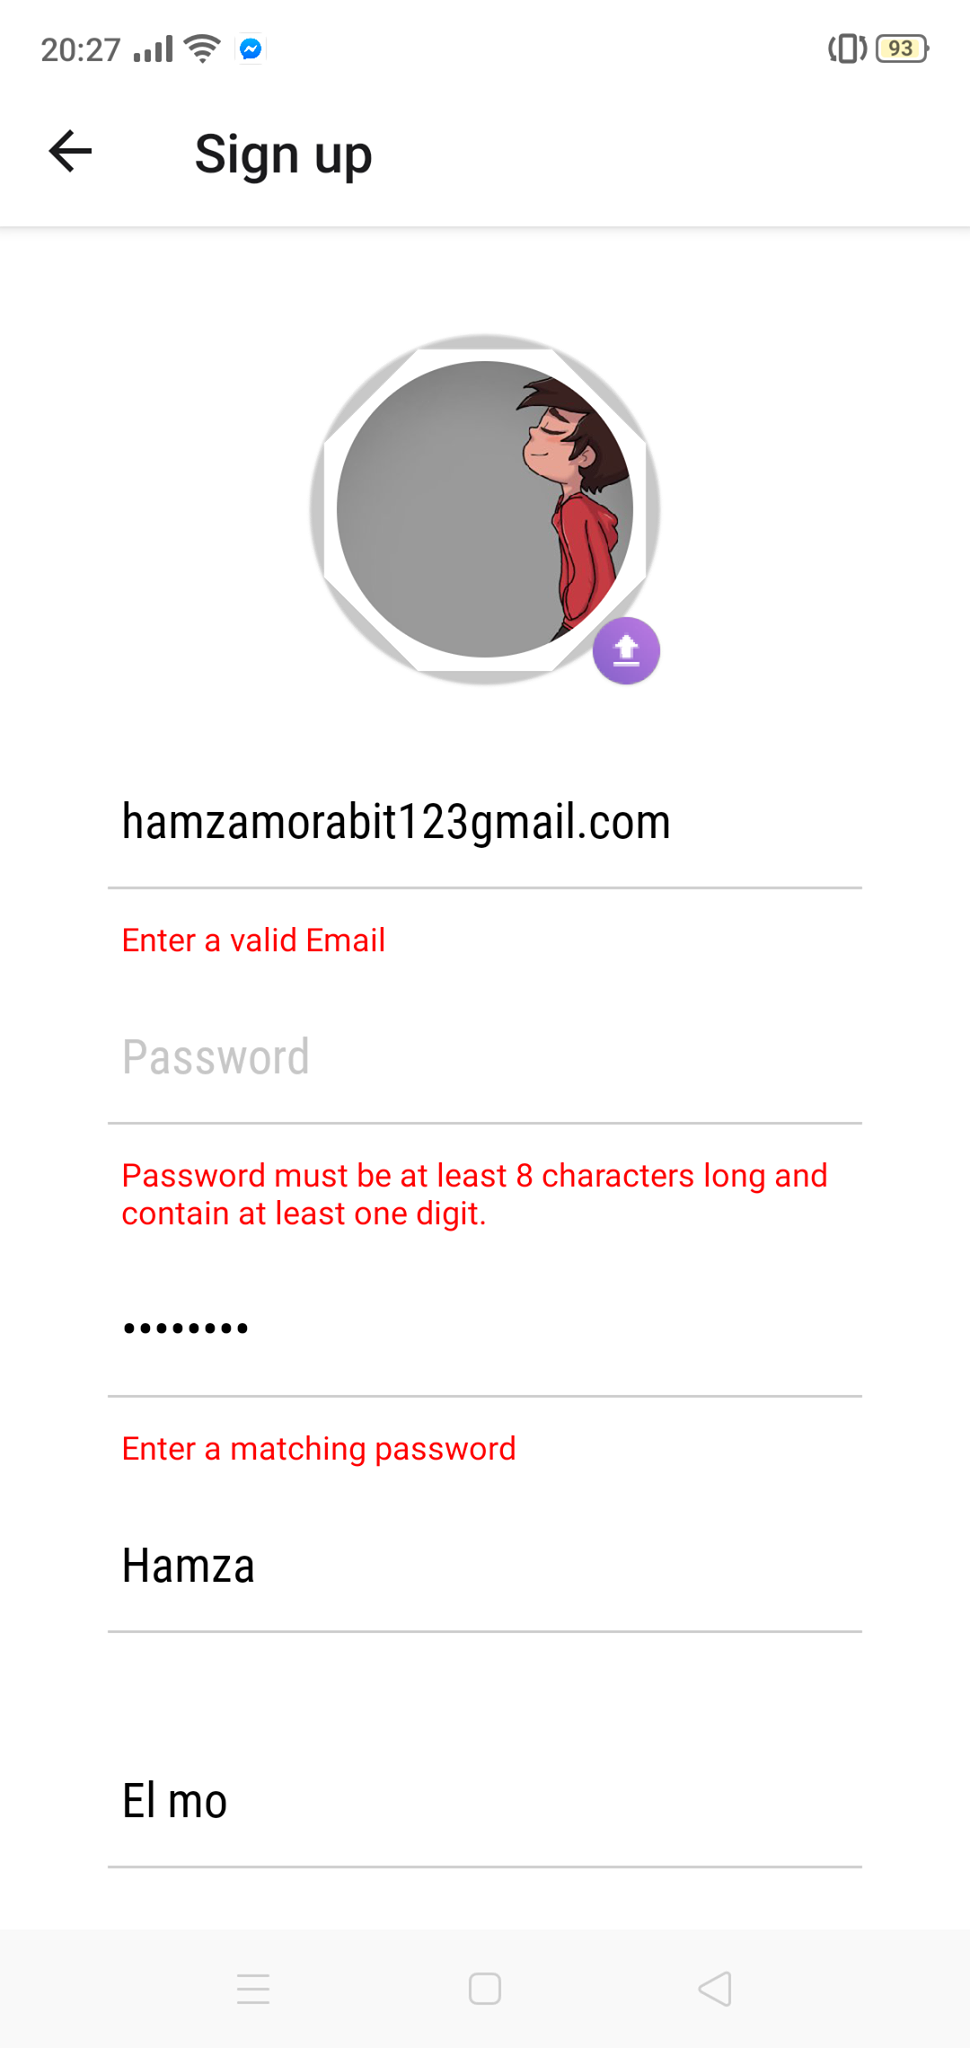
\includegraphics[width=7cm,height=7cm,keepaspectratio]{Application/insc1.png} 
% \caption{Interface d'inscription pour choisir type d'utilisteur}
% \end{figure}
\begin{figure}[H]
  \centering
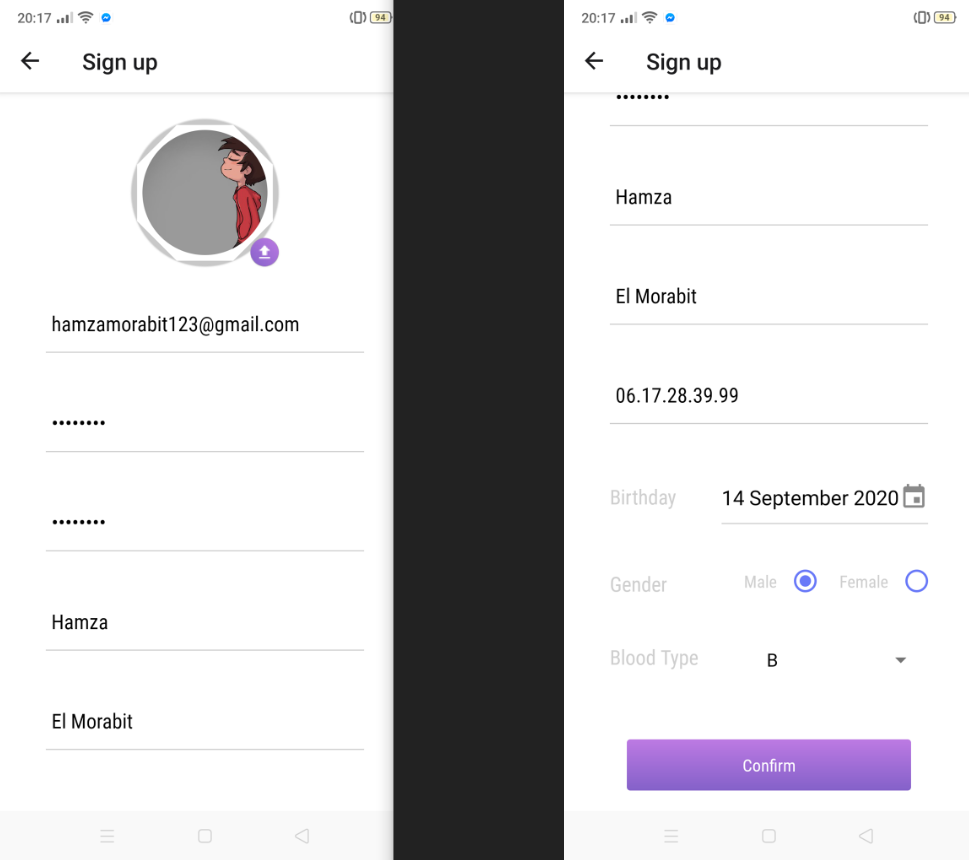
\includegraphics[width=10cm,height=8cm,keepaspectratio]{Application/med1.png} 
\caption{Interface de saisie les informations d'un nouveau compte}
\end{figure}


puis , il faut remplir tous les champs pour créer un nouveau compte sinon un message d'erreur s'affichera à l'interface comme on voit au-dessous .
\begin{figure}[H]
  \centering
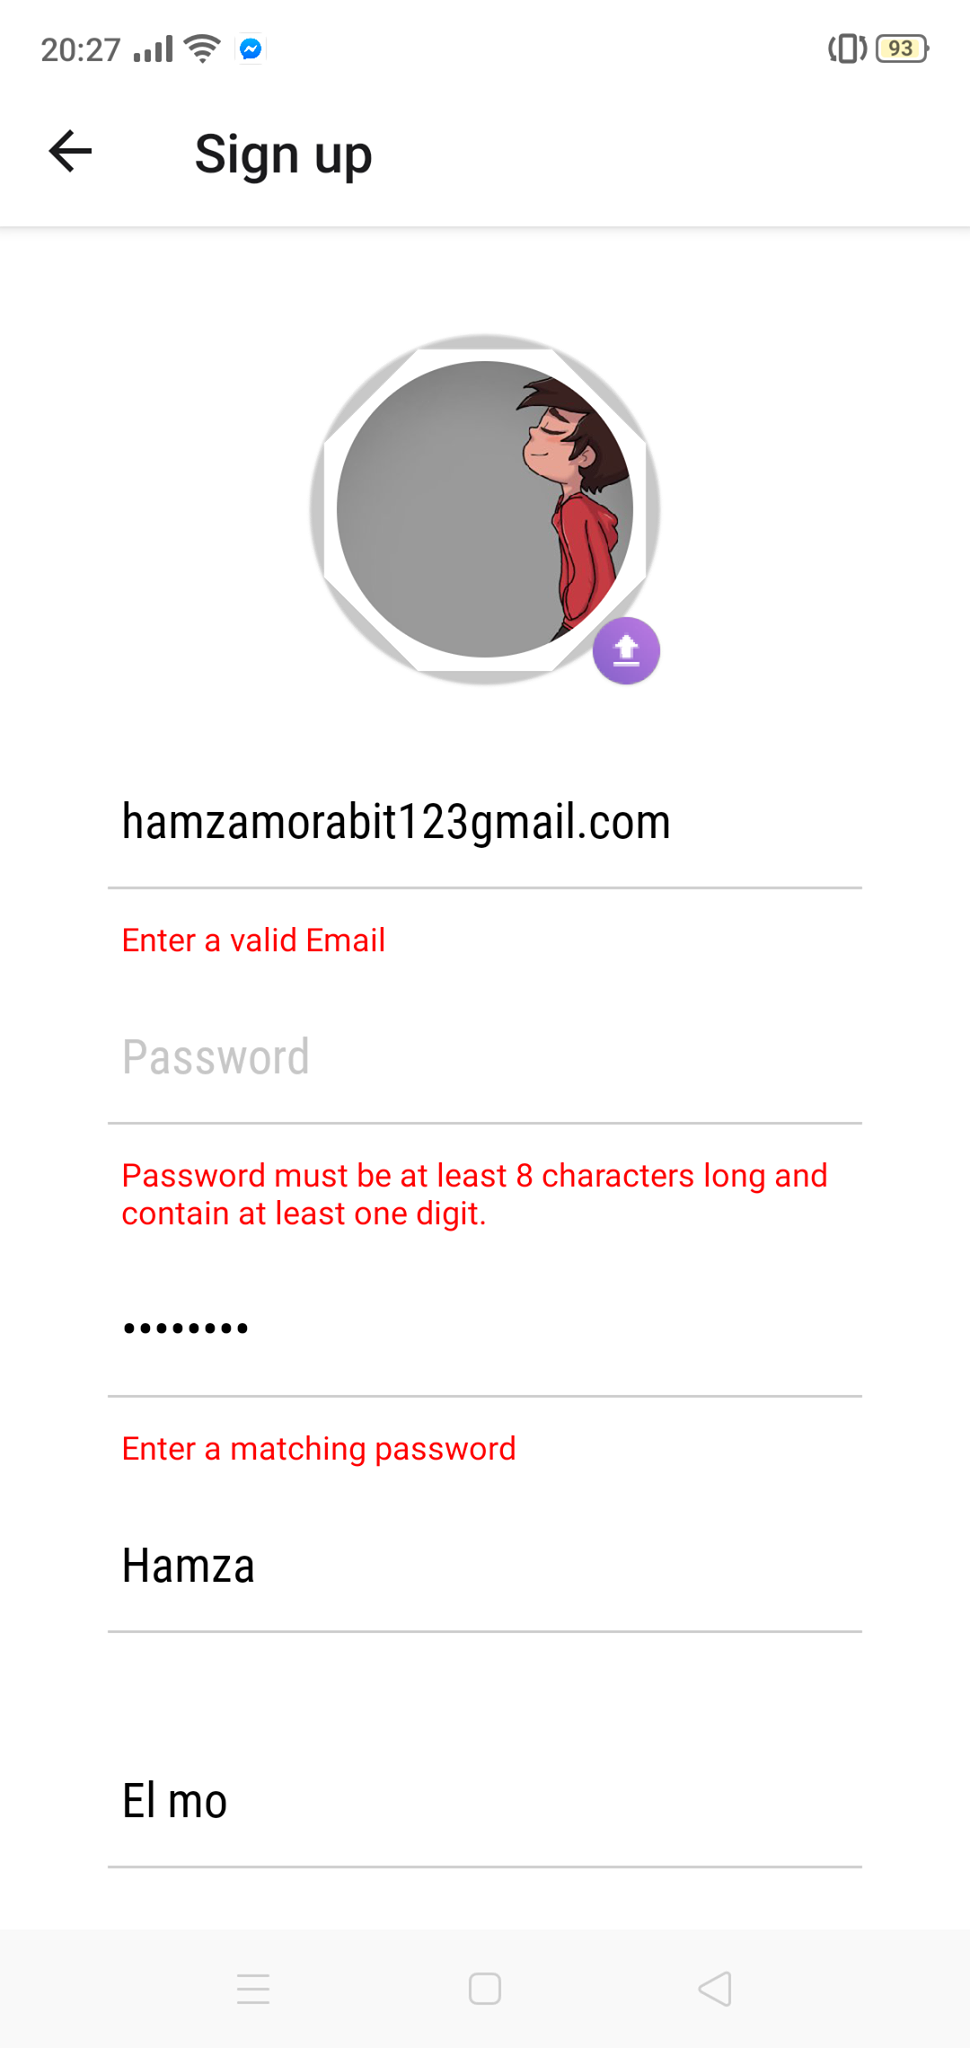
\includegraphics[width=8cm,height=8cm,keepaspectratio]{Application/insc1.png} 
\caption{Interface de saisie les informations d'un nouveau compte en cas d'erreur}
\end{figure}




\section{Consulter la profile }
\begin{figure}[H]
  \centering
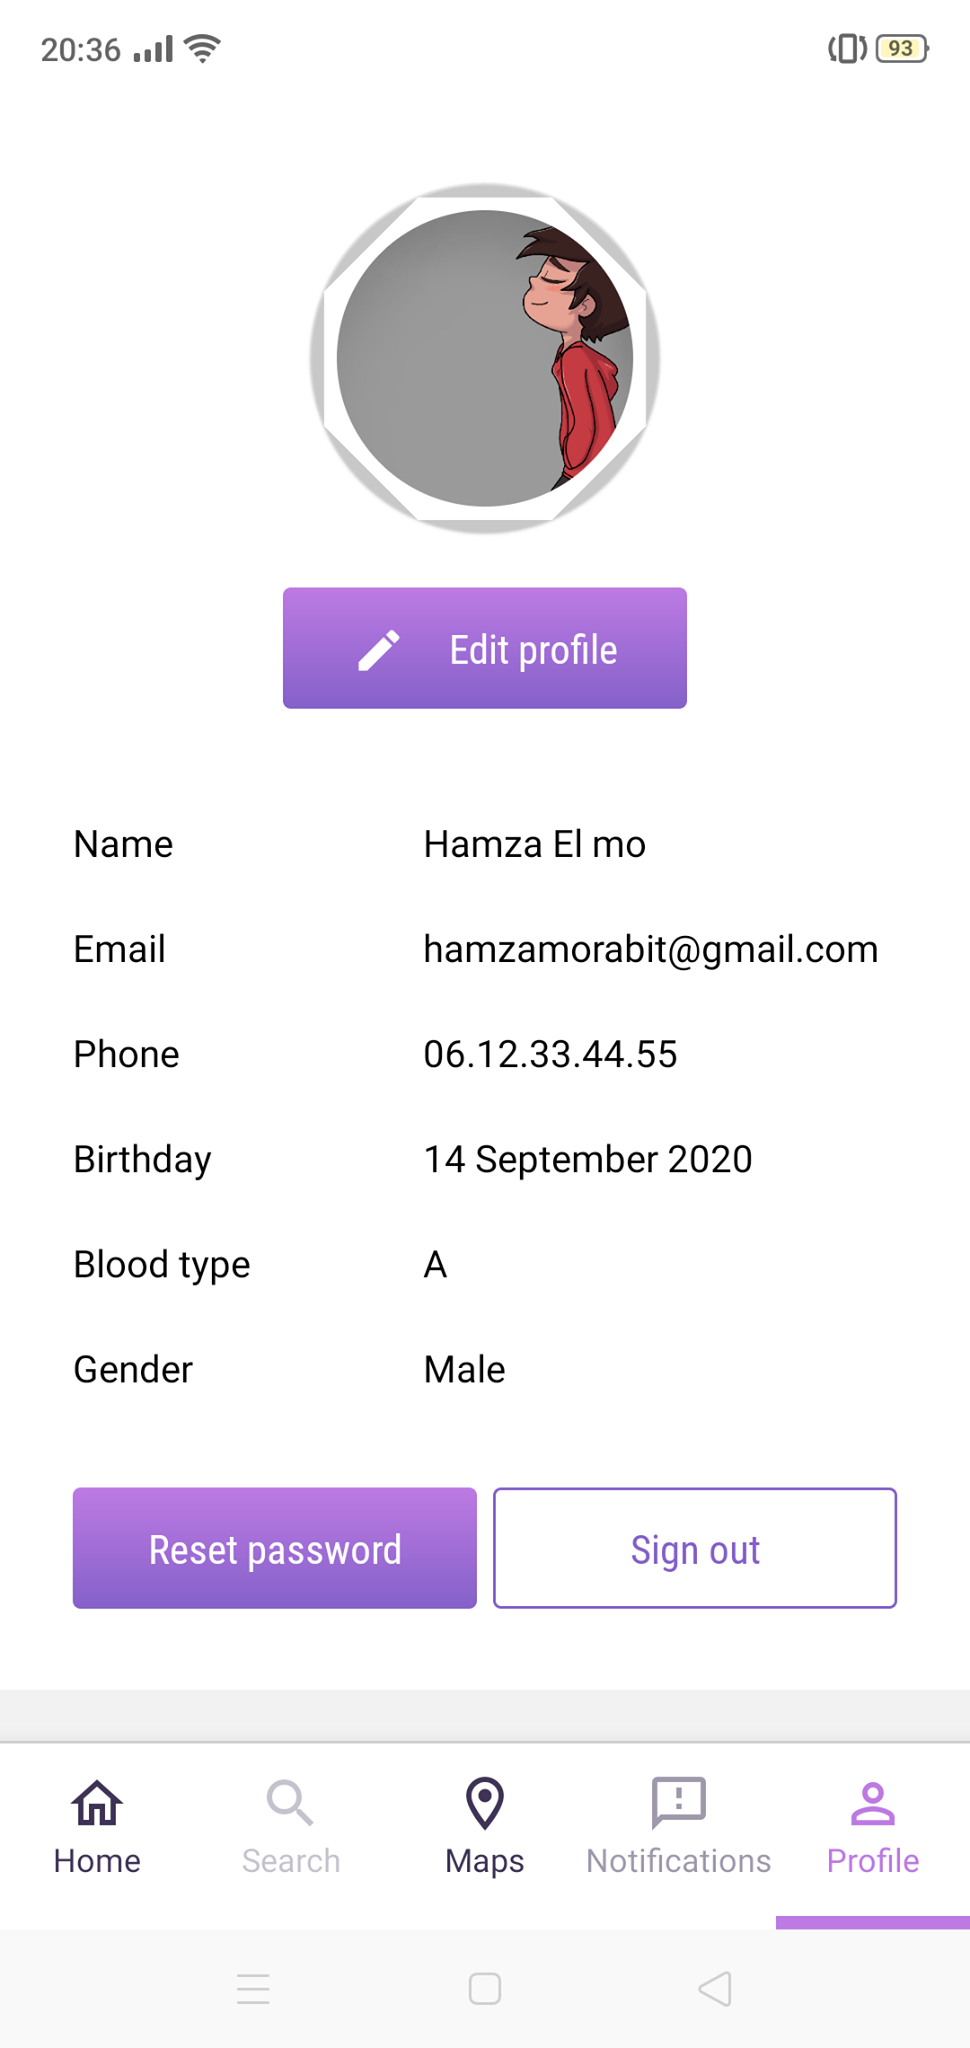
\includegraphics[width=10cm,height=8cm,keepaspectratio]{Application/med22.png} 
\caption{Interface de  consulter le profil}
\end{figure}


Cette interface contient des champs textes dans lesquels il y'a les informations que l'utilisateur a déja insérer en création du compte.
Les champs ne sont pas éditables, on ne peut pas les modifier seulement si on clique sur la boutton 'Edit profil', dans ce cas là les champs deviennent éditables ( indiqué ci-dessous ).
Tous les modifications seront modifier aussi à la base de données.
\begin{figure}[H]
  \centering
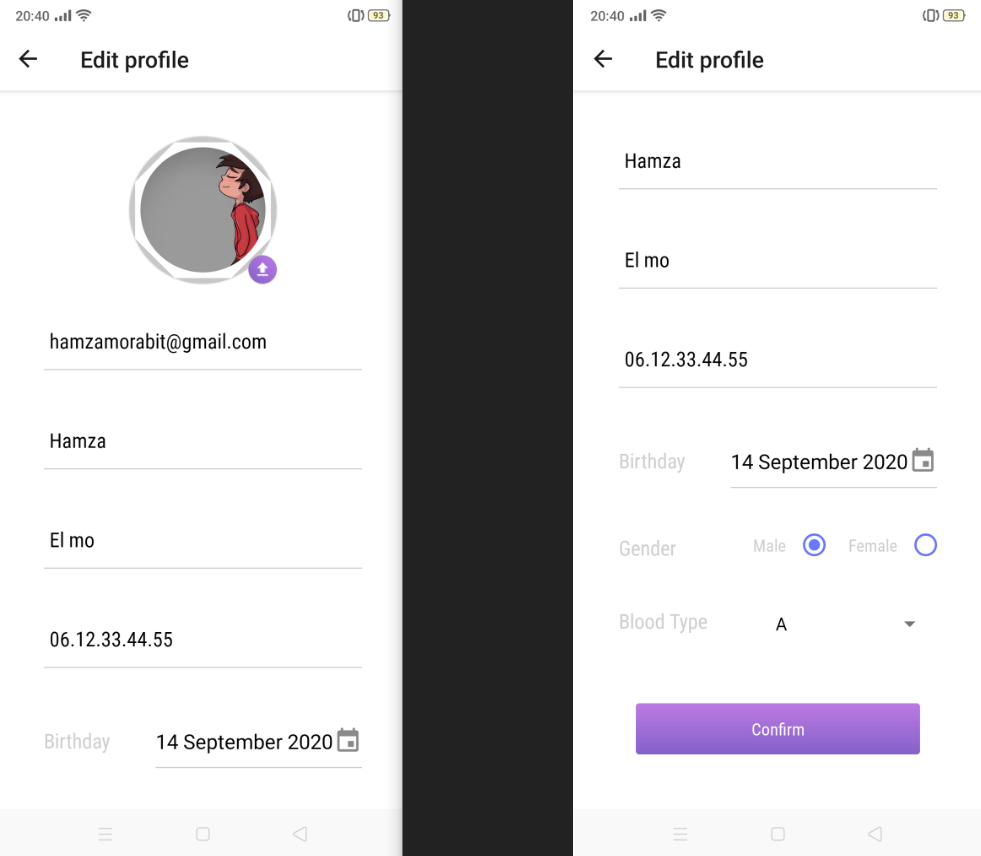
\includegraphics[width=10cm,height=8cm,keepaspectratio]{Application/medd.png} 
\caption{Interface de modifier le profil}
\end{figure}

\section*{Page d’accueil }
\begin{figure}[H]
  \centering
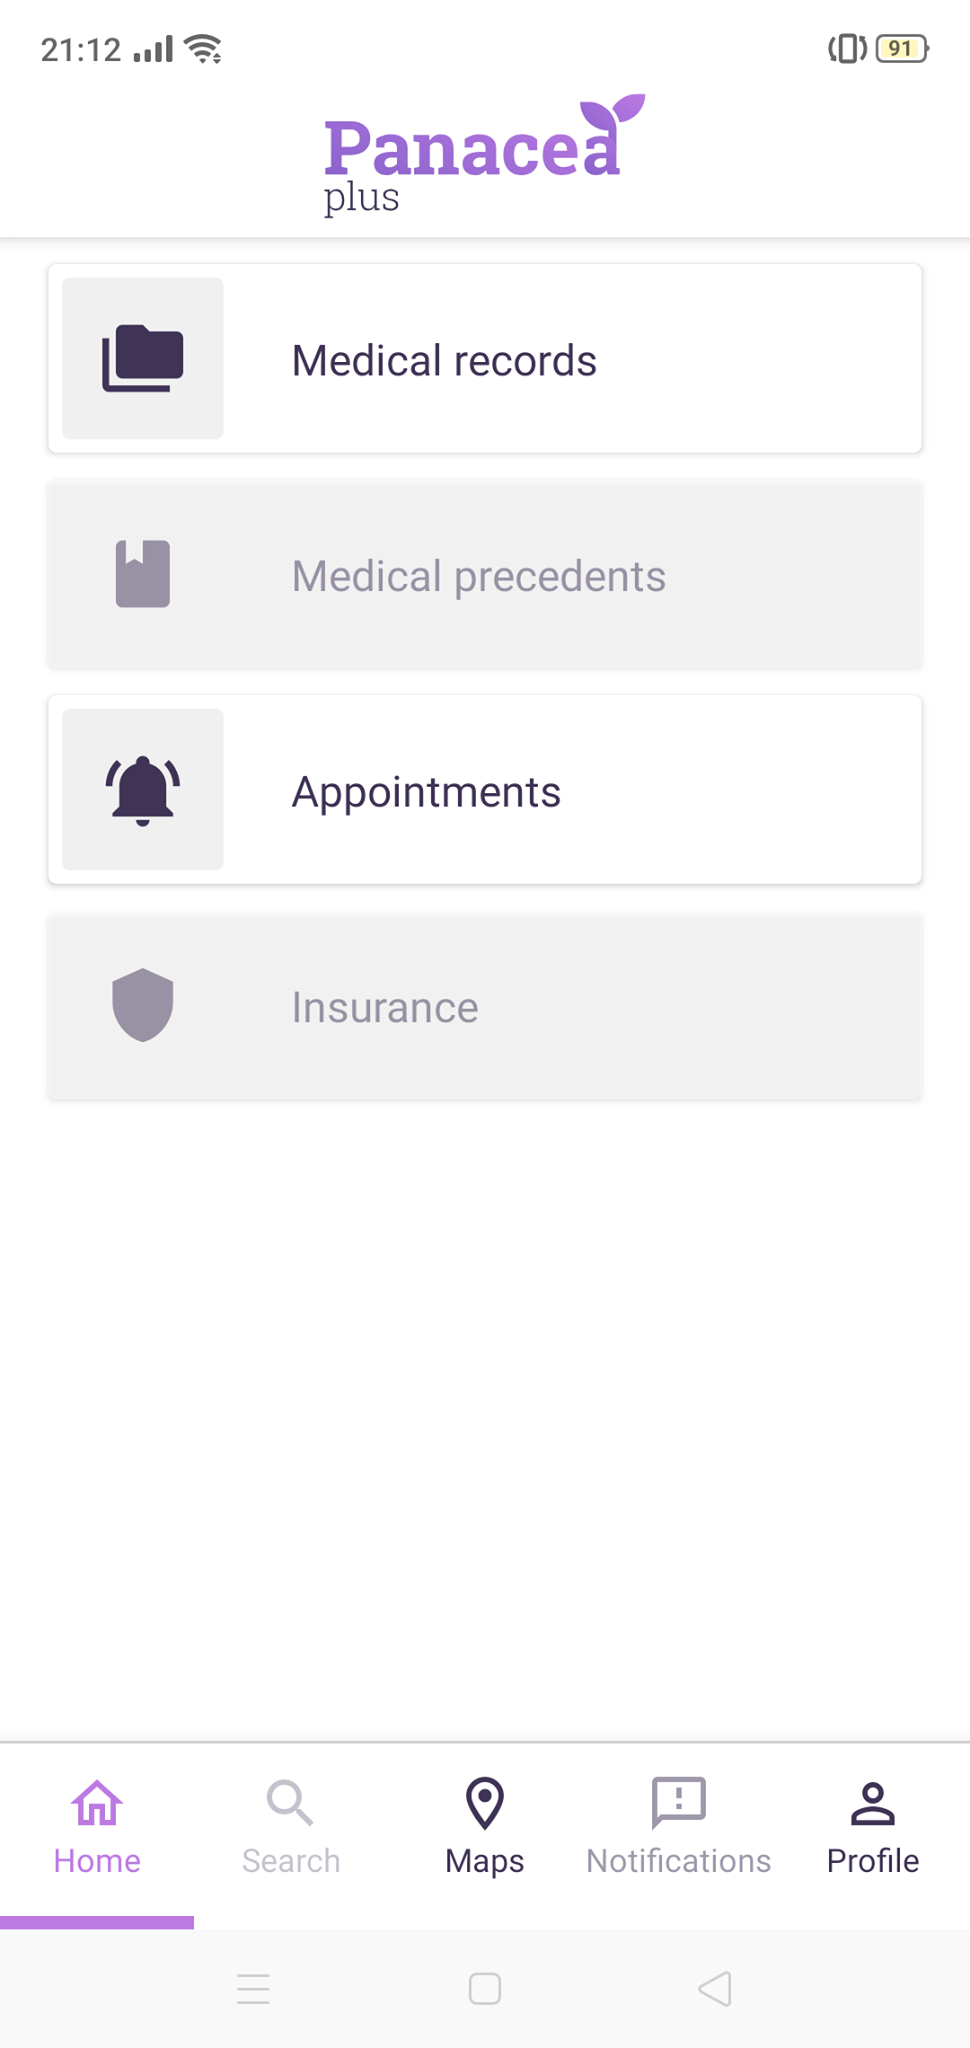
\includegraphics[width=9cm,height=7cm,keepaspectratio]{Application/acc.png} 
\caption{Menu de l'application}
\end{figure}



% \section{Des interfaces du patient }
\subsection{Réinitialiser Mot de Passe }
La figure ci-dessus montre la page d’accueil qui va apparaitre dès que l'utilisateur appuie sur 'resetPassword'  . Cette interface  à un rôle très un important parfois l'utilisateur à oublier son code l'utilisateur il a cette  solution pour récupérer leur code car celle-ci fonctionnera d'une façon sécurisée 
\begin{figure}[H]
  \centering
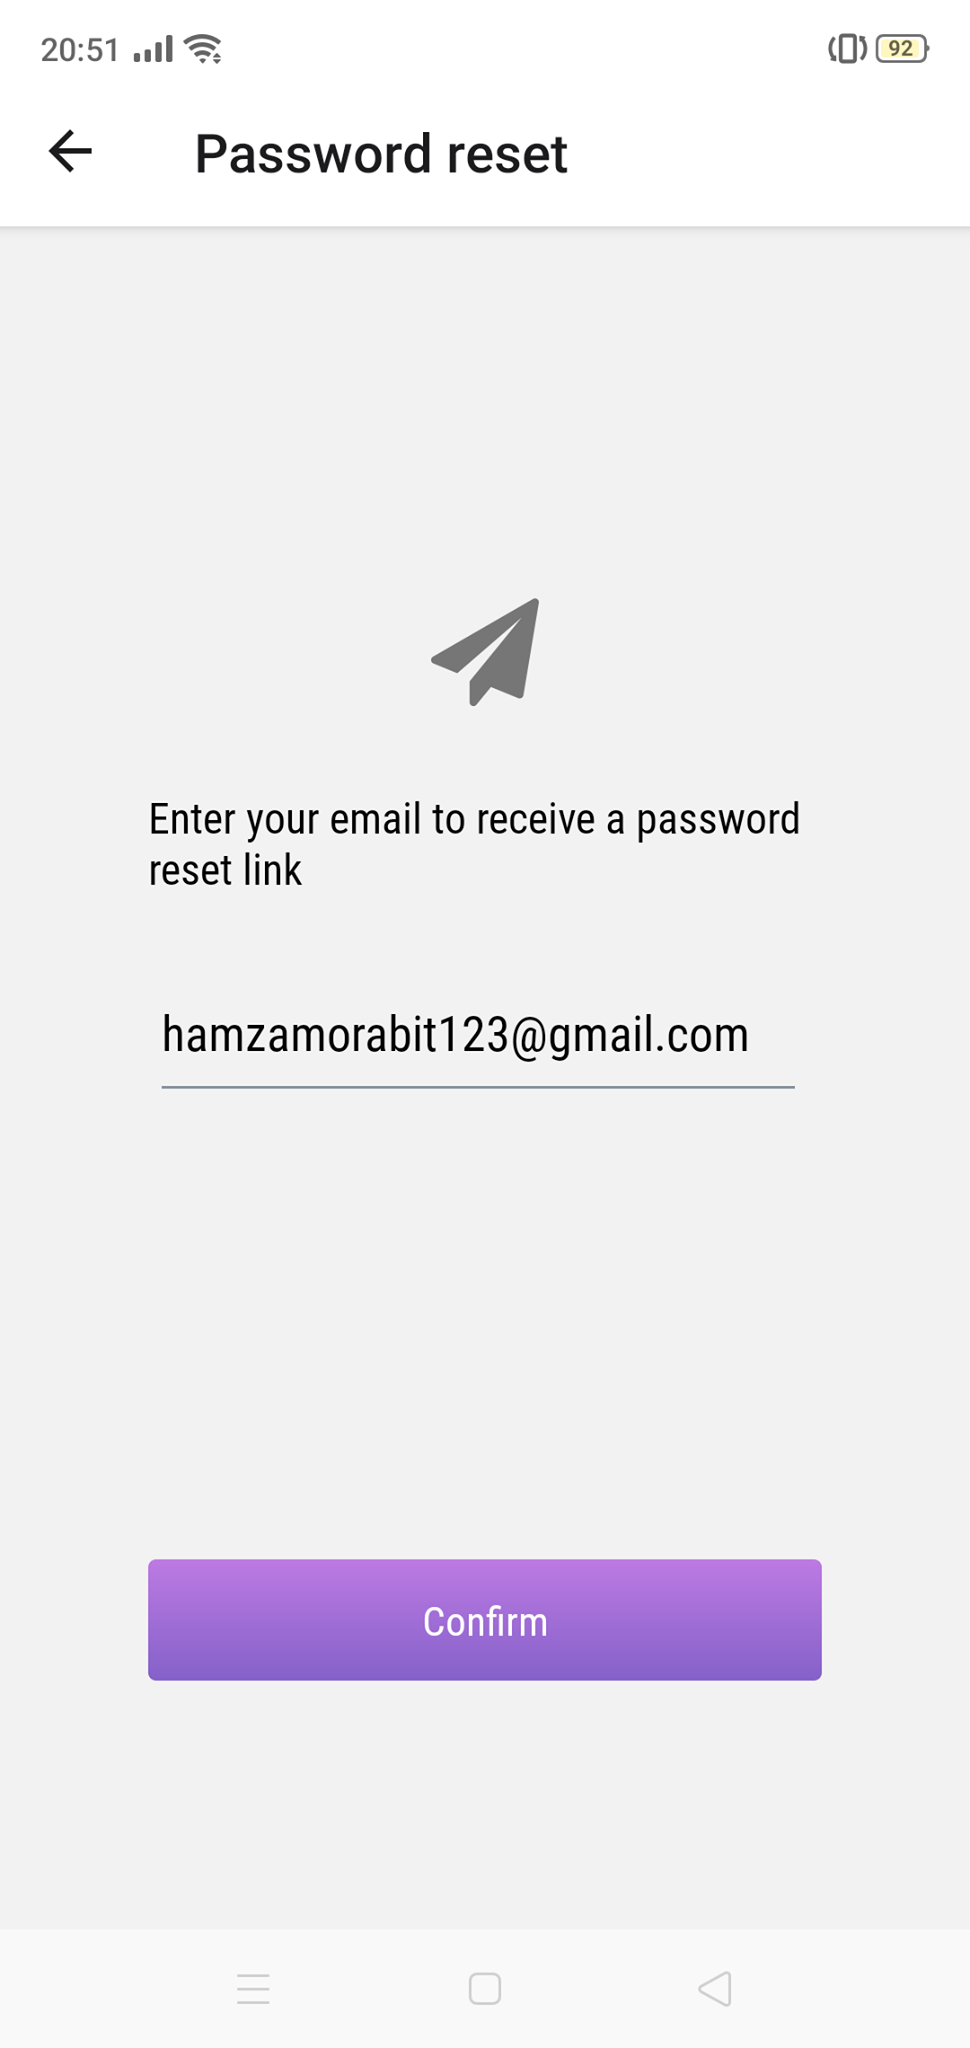
\includegraphics[width=9cm,height=7cm,keepaspectratio]{Application/err2.png}
\caption{Interface de réinitialiser Mot de Passe}
\end{figure}
Si L'utilisateur a saisi un mail qui ni correct ni dans la base de données l'interface dirige l'utilisateur sur une autre   interface (ci-dessous)
\begin{figure}[H]
  \centering
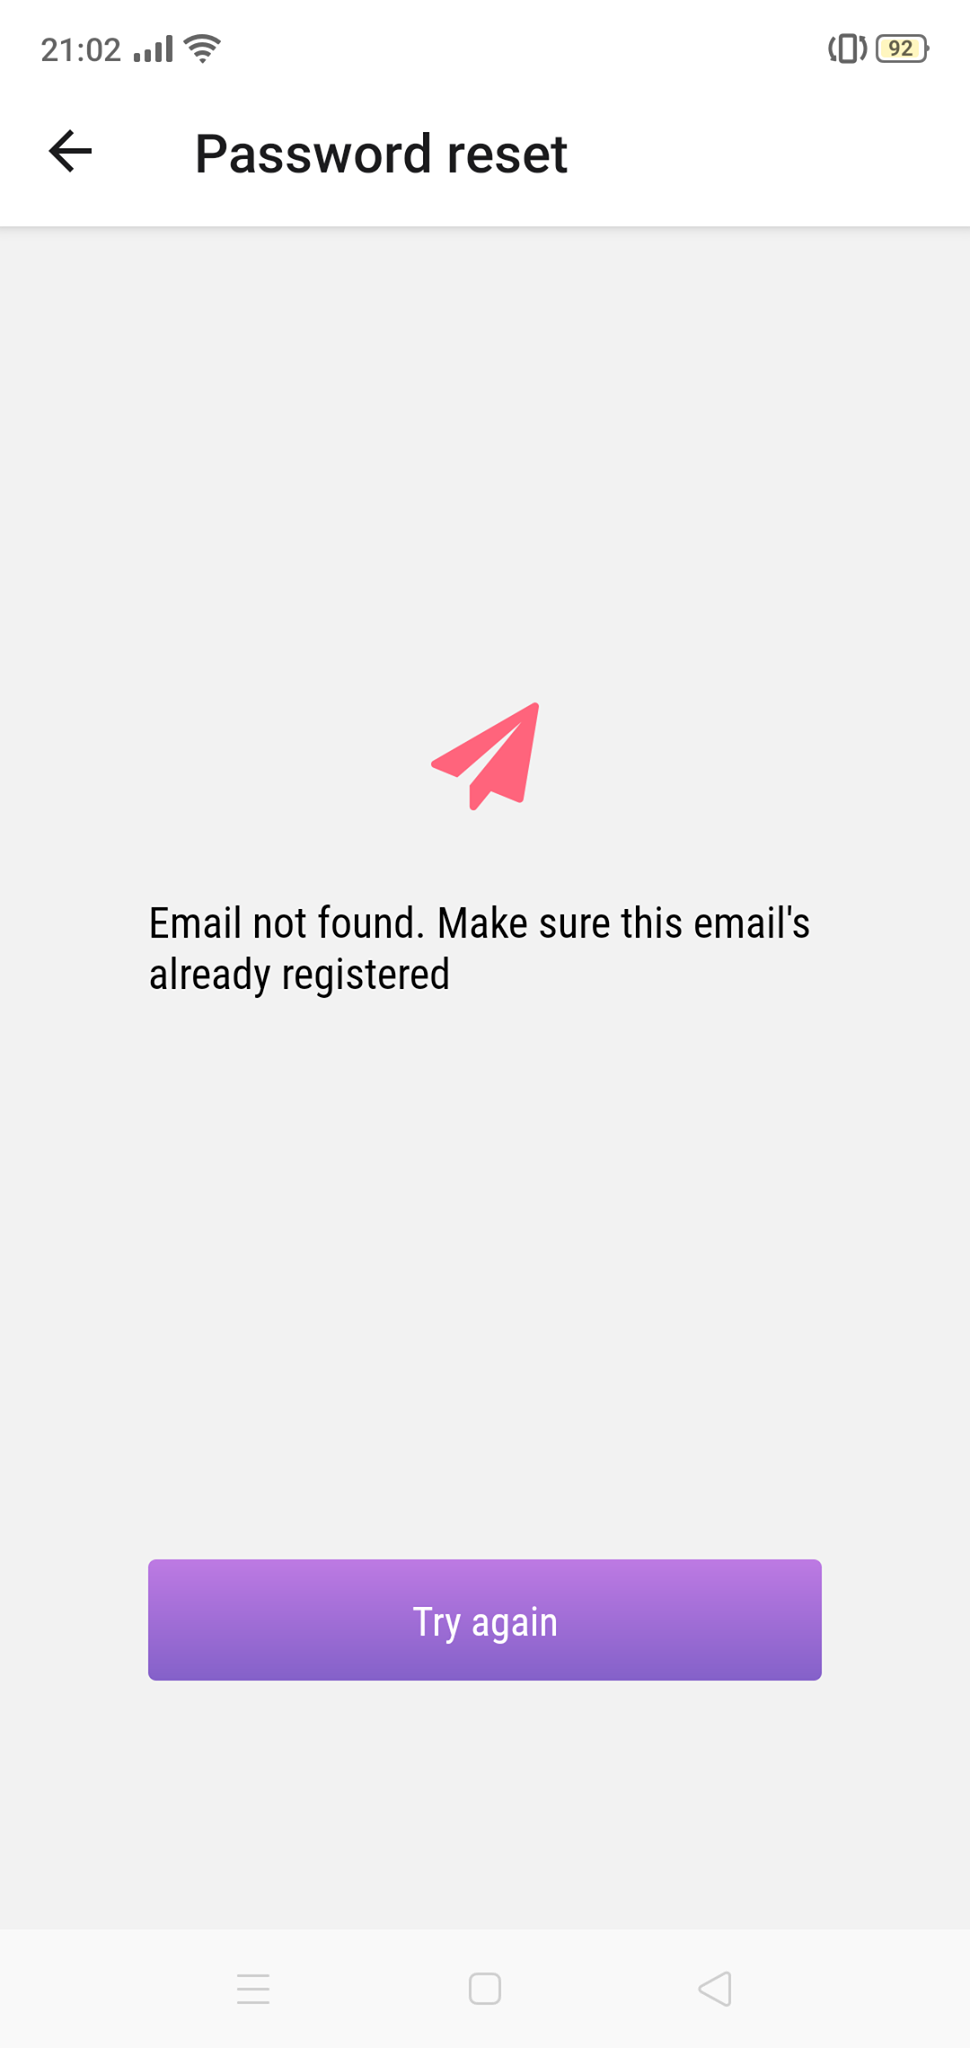
\includegraphics[width=9cm,height=7cm,keepaspectratio]{Application/ert.png}
\caption{Interface de réinitialiser Mot de Passe en cas d'erreur}
\end{figure}



\subsection{Rendez-vous}
Permet de programmer les rendez-vous et comprend aussi bien :\\
* programmation des visits à effectué aux docteurs .\\
* Remarque des docteurs ( orodonnace pharmacetique , d'analyse ..)\\
* La date 
\begin{figure}[H]
  \centering
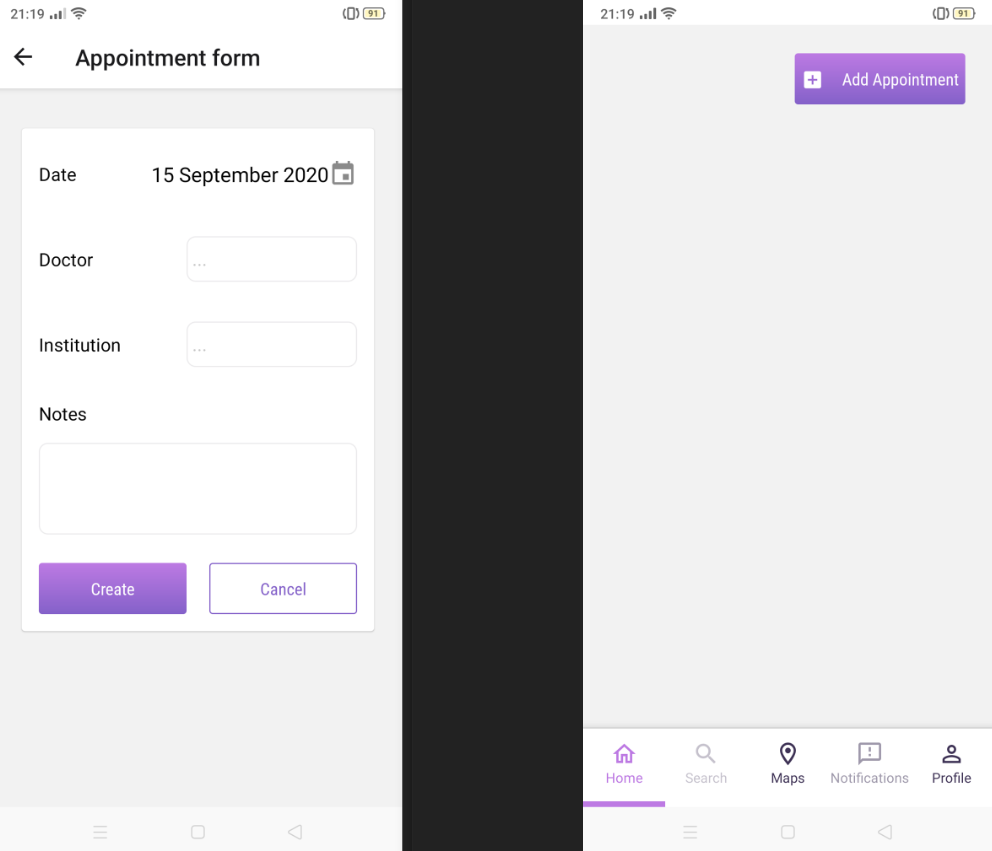
\includegraphics[width=9cm,height=7cm,keepaspectratio]{Application/app0.png} 
\caption{Interface de prendre un rendez-vous}
\end{figure}
L'application permet aussi à l'utilisateur de modifier ou supprimer certain rendez-vous
\subsection{Recherche l’emplacement}
La carte (Maps) permet de choisir et localiser les cabinets les plus proches et faciliter l'accessibilité

\begin{figure}[H]
  \centering
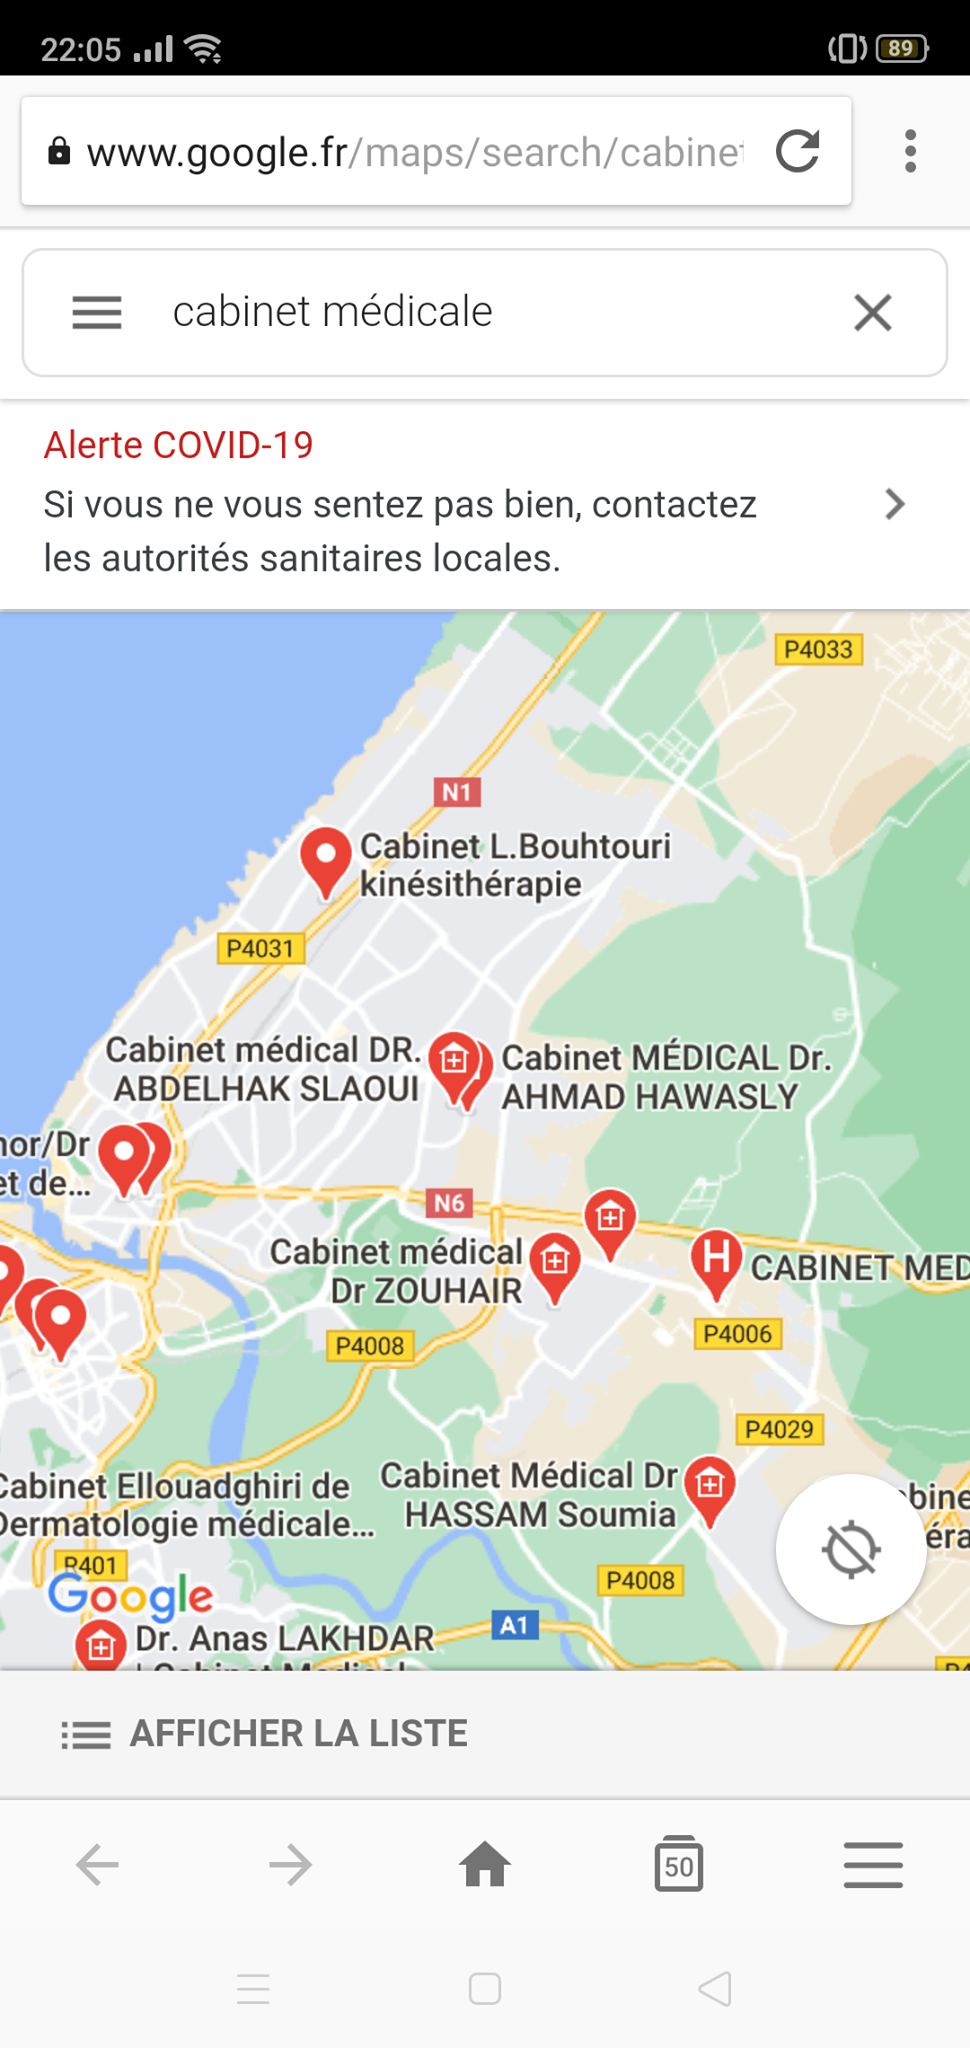
\includegraphics[width=9cm,height=8cm,keepaspectratio]{Application/map.png} 
\caption{Indiqué les  cabinets les plus proche}
\end{figure}
pour accéder à cette carte il faut d'abord avoir l'accord à sa demande

\begin{figure}[H]
  \centering
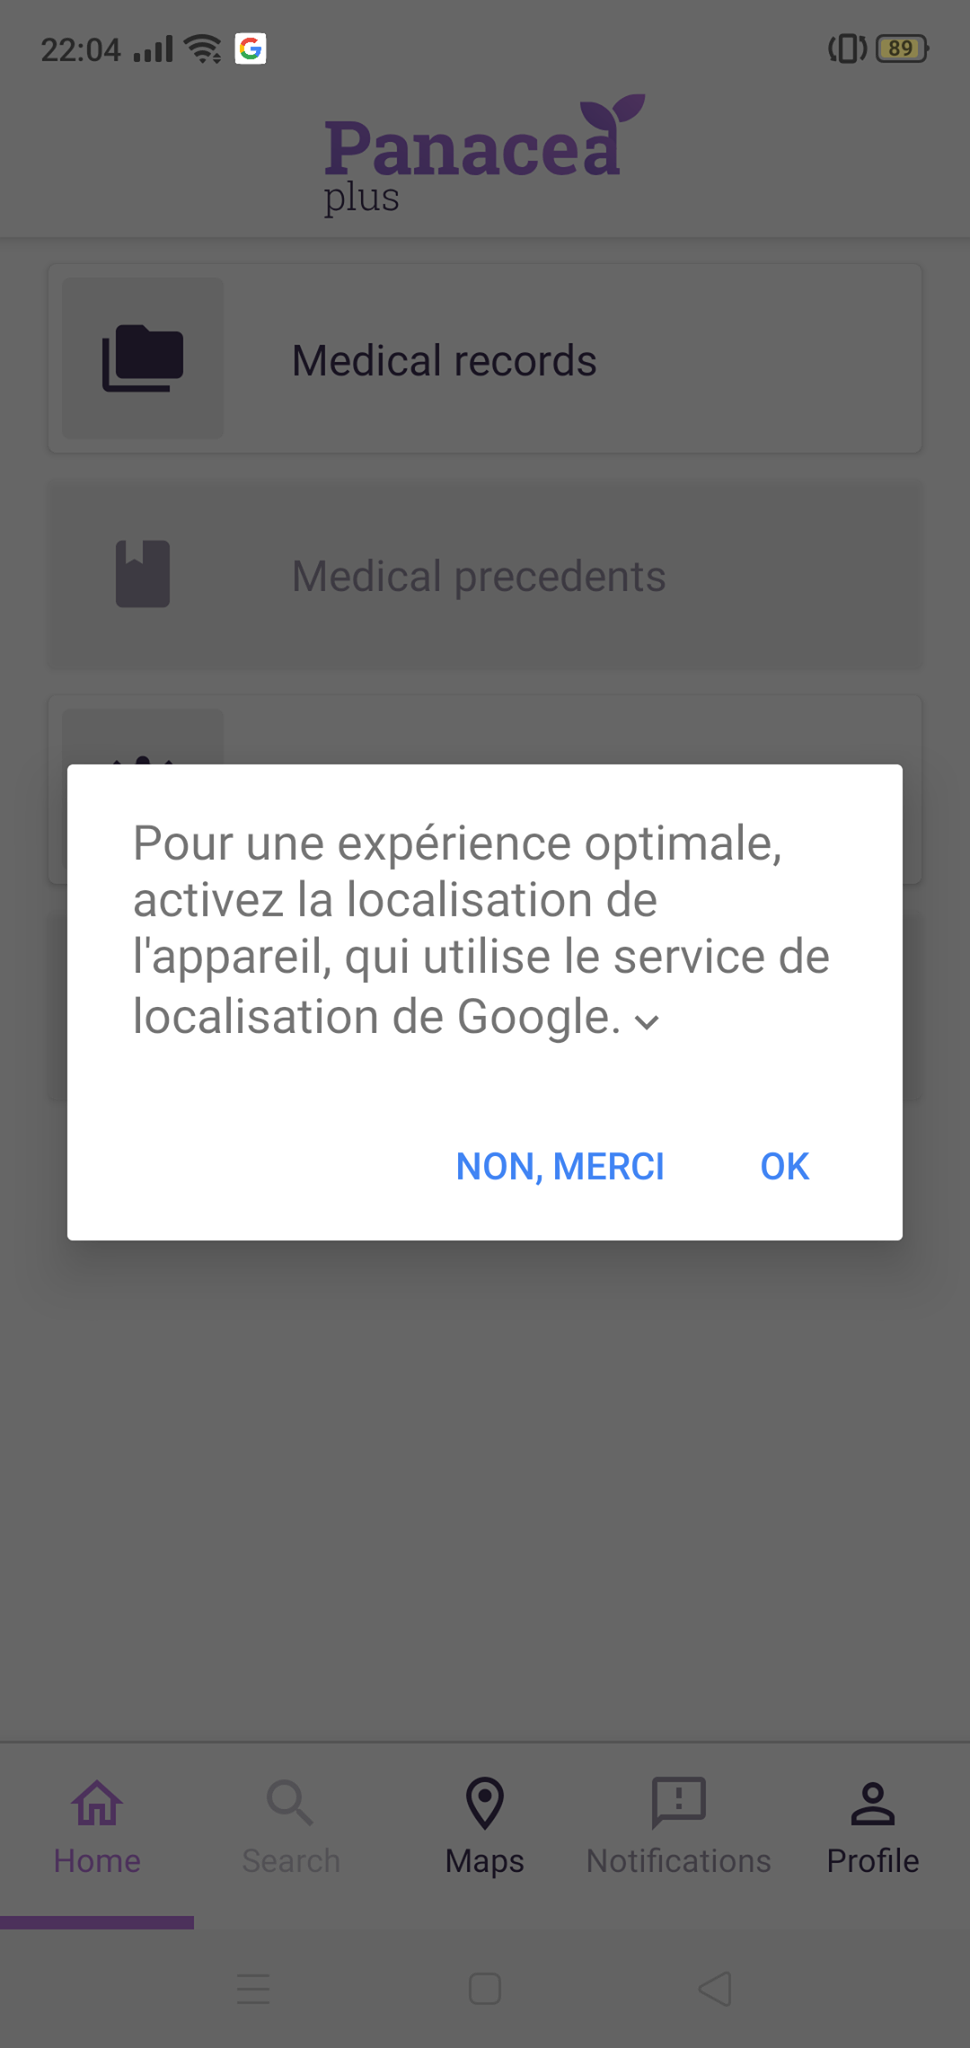
\includegraphics[width=9cm,height=8cm,keepaspectratio]{Application/auto.png} 
\caption{Interface affichage d'un messge d'accessibilité}
\end{figure}
 \subsection{Rapports médicaux }

  \subsubsection{problème cardiaque}
  Cette interface me permet d'enregistrer et de modifier  le rapport et le bilan cardiaque du docteur
  \begin{figure}[H]
  \centering
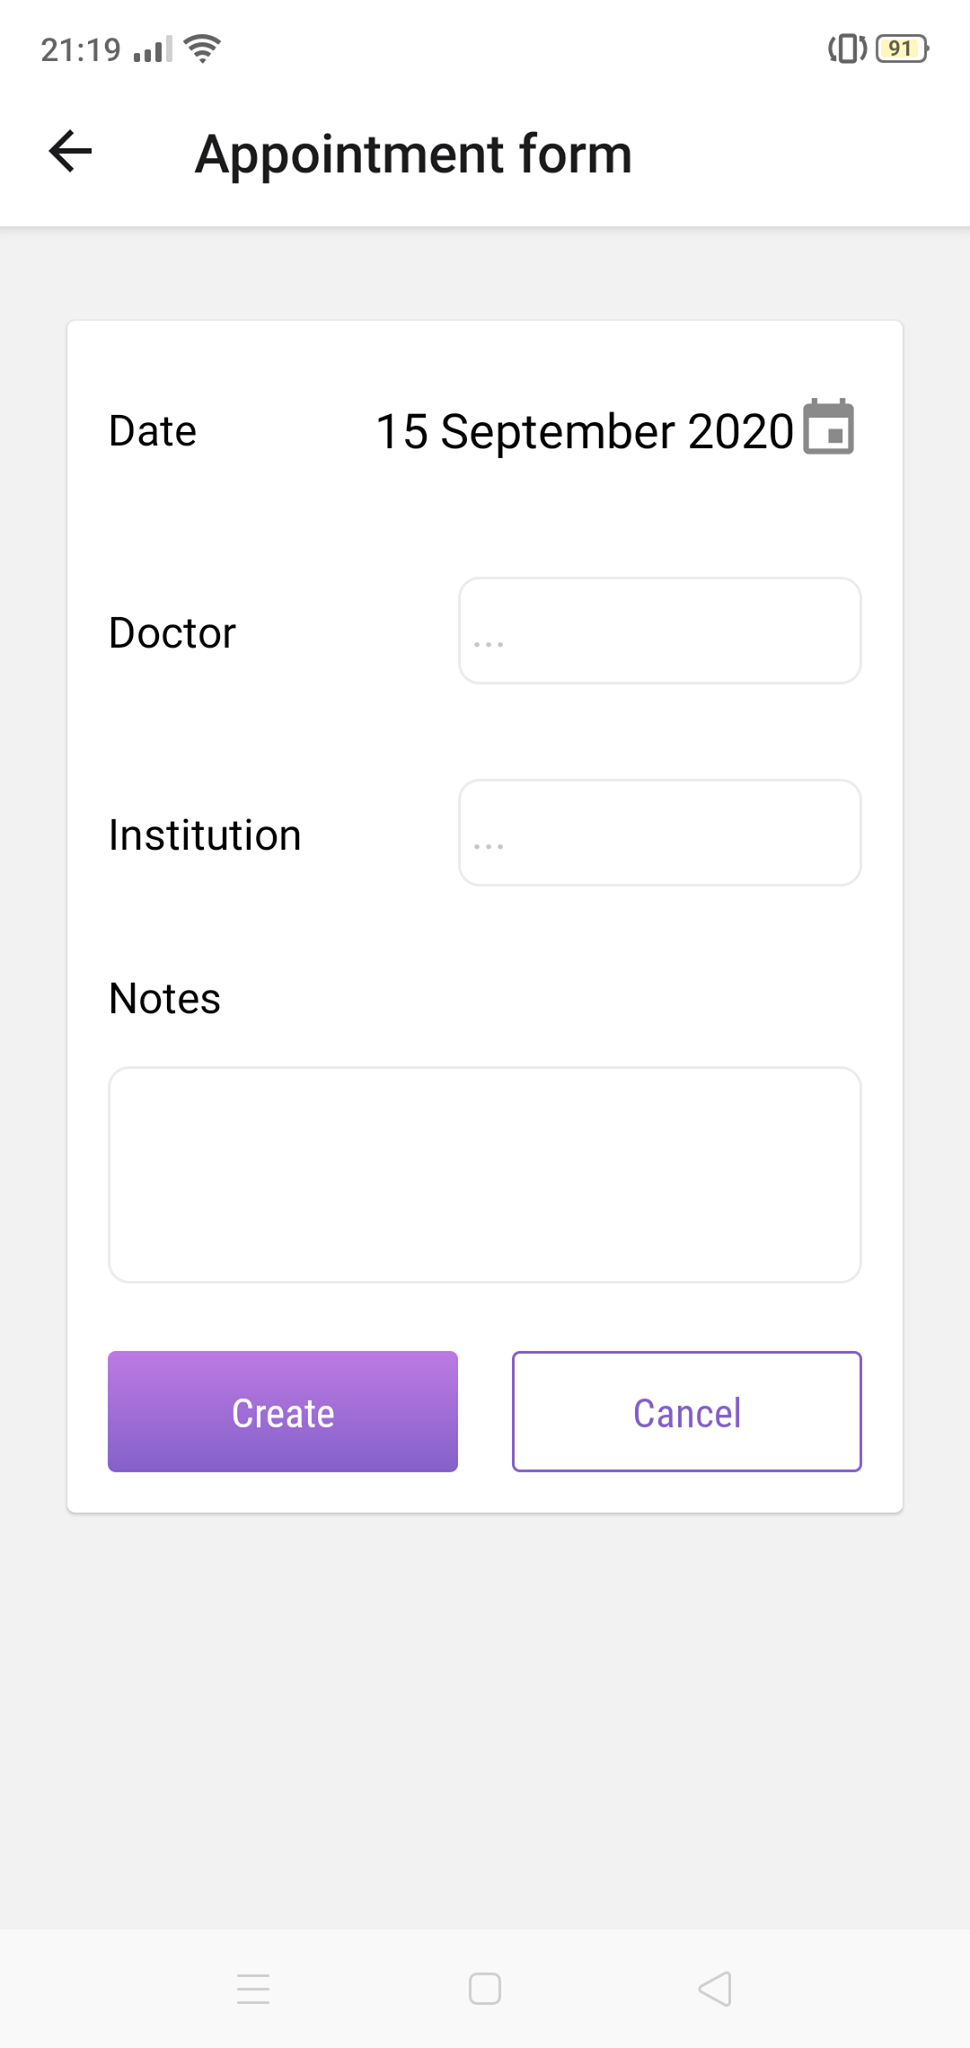
\includegraphics[width=9cm,height=8cm,keepaspectratio]{Application/bil.png} 
\caption{Interface affichage d'un messge d'accessibilité }
\end{figure}
% % cette fragement contient les informations personelle du patient et les valeurs du paramètres vitaux (Taille,Poids,Temperature,Pouls,Respiration,Glycemie capillaire,Tension et groupe sanguin).
% \subsection*{Diagnostic:}
% \begin{figure}[H]
%   \centering
% 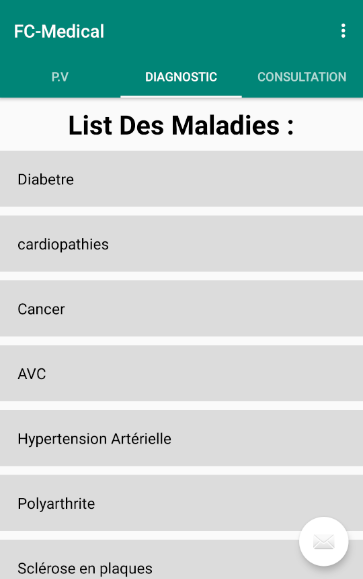
\includegraphics[width=7cm,height=7cm,keepaspectratio]{Application/dossier3.png} 
% \caption{ Interface de Diagnostic}
% \end{figure}

% Contient diagnostic de ces maladies suivants (Diabète, cardiopathies, cancer, AVC, hypertension artérielle, polyarthrite, sclérose en plaques, maladie de Crohn).
% \subsection*{Consultation : }
% \begin{figure}[H]
%   \centering
% 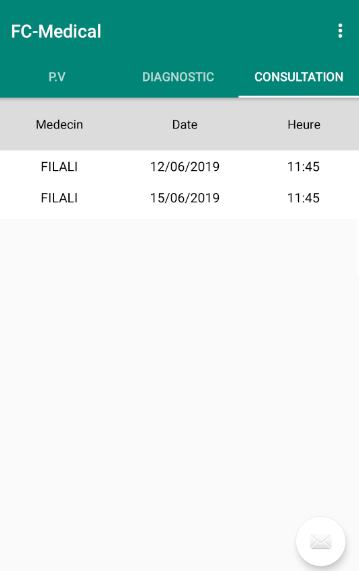
\includegraphics[width=7cm,height=7cm,keepaspectratio]{Application/dossier5.png}
% \caption{ Interface de Consultation}
% \end{figure}

% Contient les Rendez-vous que le patient a avec un médecin
% \subsection{Interface de Traitement }
% \begin{figure}[H]
%   \centering
% 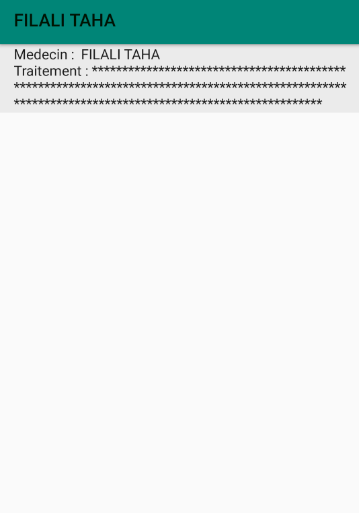
\includegraphics[width=7cm,height=7cm,keepaspectratio]{Application/trait1.png} 
% \caption{ Interface de Traitement}
% \end{figure}

% Cette interface contient les mesures appliquées par le médecin au patient afin de l'aider à en guérir, de soulager ses symptômes, ou encore d'en prévenir l'apparition.

% Si Le patient n'a pas un dossier médicale une boite dialog s'affiche pour demender au patient s'il vaut creér un maintenant ou non.
% \begin{figure}[H]
%   \centering
% 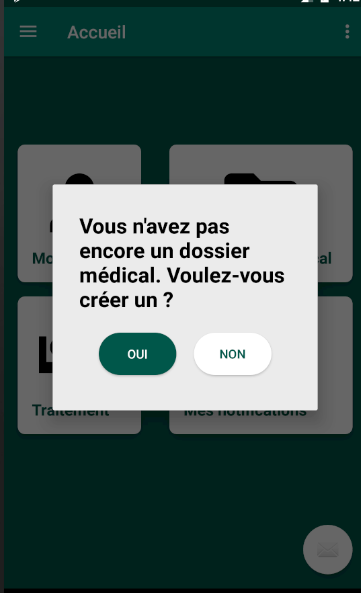
\includegraphics[width=8cm,height=8cm,keepaspectratio]{Application/dossier8.png} 
% \caption{ Interface de demender de creation un dossier médicale}
% \end{figure}

% \newpage
% \section{Les interfaces du medécin }
% \subsection{Interface d'accueil }
% \begin{figure}[H]
%   \centering
% 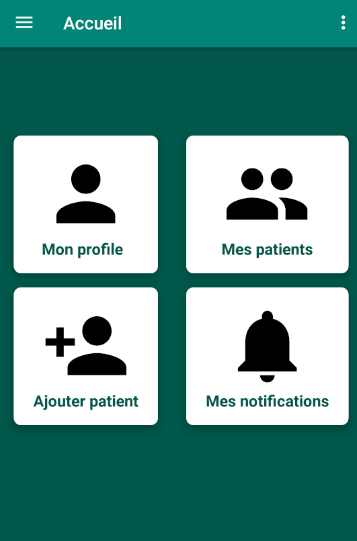
\includegraphics[width=7cm,height=7cm,keepaspectratio]{Application/medecin1.png} 
% \caption{ Interface de d'acceuil du medécin}
% \end{figure}

% Cette figure ci-dessus montre la page d’accueil qui va apparaitre dès qu’un médecin lance l’application après s'authentification  . Cet interface comporte un GridView contient  4 figures sont  "Mon Profil" ,"Mes patients","Ajouter patient" et "Mes Notification" , qui en cliquant sur une figure , va nous diriger vers L'interface que nous avons choisie  .
% rface d’accueil du patient

% \subsection{Interface de patients de medécin }
% \begin{figure}[H]
%   \centering
% 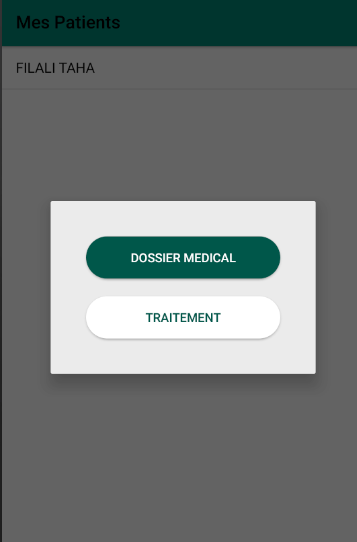
\includegraphics[width=7cm,height=7cm,keepaspectratio]{Application/mespatient1.png}
% \caption{ Interface de patients de medécin}
% \end{figure}


% En cette interface on aura une liste des patients que le médecin suive.
% En cliquant sur un élément,une boite de dialogue s'affichera et nous demande de choiser si aller vers le dossier medical du patient pour le consulter ou le modifier,si aller vers l'interface du traitement ou le médecin peut saisir le traitement que le patient doit suivre.


% \subsection{Interface d'ajouter un patient}
% \begin{figure}[H]
%   \centering
% 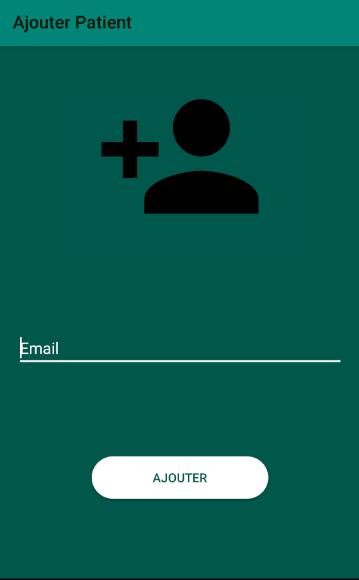
\includegraphics[width=7cm,height=7cm,keepaspectratio]{Application/ajo2.png} 
% \caption{Interface d'ajouter un patient}
% \end{figure}

% Dans cette interface le médecin peut envoyer une invitation par saisir l'email du patient requis.


\section*{conclusion }
Ce chapitre décrit les interfaces graphique du l'application et ses fonctionnements qui sont utilisés par l'utilisateur . 

\newpage

\chapter{Conclusion et perspectives}
{\large


%   Au bout de notre cursus en licence informatique, nous avons été chargés de réaliser un
% projet de fin d'étude. 
Notre travail s'est basé  sur la réalisation d'une application mobile médicale .
 L'application que nous avons réalisé permet à l'utilisateur d'apporter à son carnet médical les évènement  qui peut servenir et de sauvegarder les rapport et  
 les bilans médicaux d'une façon simple\\

%  , apporter des modifications aux son carnet médical
 
% au médecin de consulter et
% apporter des modifications aux dossiers médicaux de ses patients et
% etre notifier si l'un des paramètres vitaux de l'un de ses patients dépasse un seuil donné . 

La réalisation de ce projet nous a mené à explorer de nouveaux horizons de
la programmation mobile tel que le framework React Native, et FireBase ...
\\
En peut enrichir cette application de plusieurs évènement dans l'avenir
% langage de programmation ‘‘ java ’’  . \\

% Pour conclure, notre travail peut être sujet à des extensions. En effet, nous envisageons, en termes de perspectives d’ajouter la discussion directe
%  entre le patient  et son medécin sans utilser email ... , Ceci avec la
% possibilité d’être développée sous d’autres dispositifs qui utilisent d'autre systèmes d'exploitation comme Iphone.


}


\newpage

\begin{thebibliography}{10} % 0 si vous avez moins de 9 références sinon 10

\bibitem{1}
https://firebase.google.com/docs
\bibitem{2}
https://hackernoon.com/introduction-to-firebase-218a23186cd7
\bibitem{3}
https://openclassrooms.com/fr/courses/2023346-creez-des-applications-pour-android
\bibitem{4}
https://android.developpez.com/cours/

\end{thebibliography}





\end{document} 